\documentclass{article}\usepackage[table]{xcolor}
\usepackage[]{graphicx}\usepackage[table]{xcolor}
% maxwidth is the original width if it is less than linewidth
% otherwise use linewidth (to make sure the graphics do not exceed the margin)
\makeatletter
\def\maxwidth{ %
  \ifdim\Gin@nat@width>\linewidth
    \linewidth
  \else
    \Gin@nat@width
  \fi
}
\makeatother

\definecolor{fgcolor}{rgb}{0.345, 0.345, 0.345}
\newcommand{\hlnum}[1]{\textcolor[rgb]{0.686,0.059,0.569}{#1}}%
\newcommand{\hlstr}[1]{\textcolor[rgb]{0.192,0.494,0.8}{#1}}%
\newcommand{\hlcom}[1]{\textcolor[rgb]{0.678,0.584,0.686}{\textit{#1}}}%
\newcommand{\hlopt}[1]{\textcolor[rgb]{0,0,0}{#1}}%
\newcommand{\hlstd}[1]{\textcolor[rgb]{0.345,0.345,0.345}{#1}}%
\newcommand{\hlkwa}[1]{\textcolor[rgb]{0.161,0.373,0.58}{\textbf{#1}}}%
\newcommand{\hlkwb}[1]{\textcolor[rgb]{0.69,0.353,0.396}{#1}}%
\newcommand{\hlkwc}[1]{\textcolor[rgb]{0.333,0.667,0.333}{#1}}%
\newcommand{\hlkwd}[1]{\textcolor[rgb]{0.737,0.353,0.396}{\textbf{#1}}}%
\let\hlipl\hlkwb

\usepackage{framed}
\makeatletter
\newenvironment{kframe}{%
 \def\at@end@of@kframe{}%
 \ifinner\ifhmode%
  \def\at@end@of@kframe{\end{minipage}}%
  \begin{minipage}{\columnwidth}%
 \fi\fi%
 \def\FrameCommand##1{\hskip\@totalleftmargin \hskip-\fboxsep
 \colorbox{shadecolor}{##1}\hskip-\fboxsep
     % There is no \\@totalrightmargin, so:
     \hskip-\linewidth \hskip-\@totalleftmargin \hskip\columnwidth}%
 \MakeFramed {\advance\hsize-\width
   \@totalleftmargin\z@ \linewidth\hsize
   \@setminipage}}%
 {\par\unskip\endMakeFramed%
 \at@end@of@kframe}
\makeatother

\definecolor{shadecolor}{rgb}{.97, .97, .97}
\definecolor{messagecolor}{rgb}{0, 0, 0}
\definecolor{warningcolor}{rgb}{1, 0, 1}
\definecolor{errorcolor}{rgb}{1, 0, 0}
\newenvironment{knitrout}{}{} % an empty environment to be redefined in TeX

\usepackage{alltt}%%
\usepackage{makecell}
\usepackage{amsmath}
\usepackage{caption}
\usepackage{subcaption}
\usepackage{url}
\usepackage{booktabs}
\usepackage{longtable}
\usepackage{multirow}
\usepackage[table]{xcolor}
\usepackage[]{graphicx}
\usepackage[]{color}
\usepackage{wrapfig}
\usepackage{float}
\usepackage{colortbl}
\usepackage{pdflscape}
\usepackage{tabu}
\usepackage{threeparttable}
\newcommand{\logit}{\mathrm{logit}}
\renewcommand{\$}{$} %$ 
\usepackage[utf8]{inputenc}
\usepackage[T1]{fontenc}
\DeclareUnicodeCharacter{B1}{$\pm$}
\DeclareUnicodeCharacter{2192}{$\rightarrow$}
\usepackage{hyperref}
\topmargin -1.5cm        % read Lamport p.163
\oddsidemargin -0.6cm    % read Lamport p.163
\evensidemargin -0.6cm   % same as oddsidemargin but for left-hand pages
\textwidth 17.4cm
\textheight 23.94cm 
\setlength{\parindent}{0.5cm}
\title{Data analysis supplement to ``Challenges associated with the validation 
  of protein force-fields based on structural criteria.''}
\author{M.~Stroet, M.~Setz, T.~Lee, A.~Malde, G.~van~den~Bergen, 
  \\P.~Sykacek\footnote{The responsibility for the analyses reported 
    in this supplement lies with P.~Sykacek email: peter.sykacek@boku.ac.at}, 
  C.~Oostenbrink and Alan E. Mark}
\IfFileExists{upquote.sty}{\usepackage{upquote}}{}
\begin{document}
\maketitle
\section{Introduction} 


All calculations in this document are based on the statistics package
R version 4.1.2 (2021-11-01). %$
For improved reproducibility we provide the document source
``ff\_validation\_nlme.Rnw'' as supplement. When placed together with
the files ``Simulation\_data.csv'', ``Reference\_data.csv'' and
``pdb\_id\_lengths.csv'' in the same directory, the document source
can be processed by R and the package knitr \cite{Xie:2014, Xie:2015},
as long as all additional dependencies (availability of the R packages
``kableExtra'', ``lme4'', ``emmeans'', ``car'', ``lattice'', ``nlme''
and ``dplyr'') are met. To reproduce the pdf version of this
supplement, interested readers have to use the following commands:
\begin{knitrout}
\definecolor{shadecolor}{rgb}{0.969, 0.969, 0.969}\color{fgcolor}\begin{kframe}
\begin{alltt}
\hlcom{## in R:}
\hlkwd{library}\hlstd{(knitr)}
\hlkwd{knit}\hlstd{(}\hlstr{"ff_validation.Rnw"}\hlstd{)}
\hlcom{## on the command line:}
\hlcom{## > pdflatex ff_validation.tex}
\end{alltt}
\end{kframe}
\end{knitrout}

It should be kept in mind that optimization control in the scripts
below were set to assure that a suitably small error tolerance is
reached. In case you wish to replicate the analysis, you have to
consider that as a result of these settings {\em the knitr phase in R
  takes a considerable amount of time}.
\section{Characterization of simulated proteins}
A detailed discussion of all metrics that were calculated from
simulation outcome is provided in the main paper. From a data analysis
perspective it is however important to describe the nature of the
metrics as this is important for further statistical consideration.

\begin{center}
\begin{tabular}{l l l}
  Variable name & Term in paper& Type of metric\\
  B\_Strand: &$\beta$-strand& count metric\\
  A\_Helix: &$\alpha$-helix& count metric\\
  B\_Bridge:& bridges between two $\beta$-strands in a $\beta$-sheet& count metric \\
  ThreeTen\_Helix: & $3_{10}$-helix & count metric \\
  Pi\_Helix: & $\pi$-helix & count metric \\
  Hbond\_bb\_0.25\_120: &Hydrogen bonds& count metric\\
  SASA\_polar: & solvent accessible surface area for polar residues & positive quantity\\ 
  SASA\_nonpolar: &solvent accessible surface area for non polar residues & positive quantity\\ 
  Rgyr: &Radius of gyration & positive quantity\\
  RMSD.ADJ: &Length adjusted positional RMSD & positive quantity\\ 
  phi\_rmsd: &Angular RMSD & positive quantity\\ 
  psi\_rmsd: &Angular RMSD & positive quantity\\
  NOE\_repl\_merged: & NOE intensities & positive quantity\\
  Jvalue: &J-coupling constants& positive quantity
\end{tabular}
\end{center}

\section{Data preprocessing}
Our approach for assessing protein characteristics follows
\cite{Villa+etal:2007}, who proposed analyzing the effects of force
fields on molecular-simulation derived protein characteristics with a
MANOVA. MANOVA type analyses have the advantage of increased power of
detecting significance in case of {\em correlated} multivariate
responses. MANOVA or multivariate linear models assume that the
residuals are multivariate Gaussian distributions. 

The metrics which characterize proteins are however either counts or
positive quantities. Analysis of such data will likely result in
residuals which deviate from Gaussian distributions, thus violating
assumptions which are inherent to MANOVA and linear models. To improve
compliance with Gaussian distributed residuals, we apply Box-Cox power
transformations \cite{Box+Cox:1964} on all individual metrics before
subjecting the data to a multivariate multilevel analysis. We used to
this end the functions provided in the R package car
\cite{Fox+Weisberg:2019}. To fulfill the constraint of the Box-Cox
power transformation in the car package that values must be larger
zero we set all zero or negative values before transformation to a
value which equals $10\%$ of the smallest non zero value. This
preprocessing was motivated to allow for a multivariate analysis of
all protein characteristics in combination.
  
An additional complication arises in this particular situation with
RMSD values which are known to depend on protein size. In combination
with the unbalanced nature of the simulation experiment a protein
length could confound the algorithm effect which we wish to assess. To
avoid any chances of being mislead, we apply therefore the
normalization procedure of RMSD values that was proposed in
\cite{Carugo+Pongor:2001}, before subjecting the adjusted RMSD values
to a Box-Cox transformation as well. 

A significance analysis for pair wise differences of metric values
between force fields is supplemented by analyses which assess
differences between simulation derived and measured protein
characteristics. With measured protein characteristics we refer to
characteristics whcih are derived from experimentally determined
crystal structure. The latter result allows for judgements of the
influence of force fileds on the agreement between simulation and
measurement.
\section{MANOVA and multivariate multilevel analysis}
The analysis in this work is inspired by \cite{Villa+etal:2007}, who
proposed an analysis of the effects of force fields on
molecular-simulation derived protein characteristics. Their original
approach is based on MANOVA type analyses which have the advantage of
increased power of detecting significance in case of {\em correlated}
multivariate responses. Albeit straightforward to apply, a
conventional MANOVA has in our situation several shortcomings.
\begin{enumerate}
\item MANOVA is only applicable to complete multivariate vectors of
  protein characteristics. Including missing information requires in
  such analyses additional steps like multiple imputations.
\item Using linear model terminology, our assessment of force fields
  require to consider three effects: a) the force field, b) the
  simulated protein and c) technical replication of simulation
  runs. Technical drop outs (e.g. problems of the compute
  infrastructure) or a deliberate reduction of the number of lengthy
  simulations runs will in general cause unbalanced designs. This
  renders fixed effects analyses as in \cite{Villa+etal:2007} poorly
  specified, as unbalanced multi-effects models will in general lead
  to a dependency of p-values on the chosen type of sums of squares
  calculation (type I, II and III ANOVA).
\item An even more profound implication on our assessments of force
  fields results from the fact that the replication of simulation runs
  and the variation of simulated proteins must be considered as
  independent random effects. Fixed effects analyses have in such
  situations a general tendency to overestimate significance. Such
  situations should thus preferably be assessed with mixed effects
  models \cite{Pinheiro+Bates:2000}.
\end{enumerate}
For considering the multivariate multilevel aspect of the data, we
suggest following \cite{Snijders+Bosker:2012} pages 282 ff. To
implement their proposition in our setting, we rely on the R-nlme
package \cite{Pinheiro+Bates:2000}. In the context of multivariate
multilevel analysis, we can use a likelihood ratio test
\cite{Mood+etal:1984} to assess all metrics in combination for
significant dependencies on different force fields. Using the notion
in \cite{Snijders+Bosker:2012}, chapter 16, we have to compare an
``empty'' model which expresses the derived values of all metrics by a
metric effect and attributes all further variation to the random
effects ``protein'' and ``simulation run''. The more complex
alternative hypothesis considers ``force field'' and interactions
between ``force field'' and ``metric'' as additional fixed effects. A
subsequent assessment of the likelihood ratio of these two models
provides the required p-value for assessing the molecular simulation
derived protein characteristics for significant dependencies on
``force field''.
\subsection{Multivariate multilevel analysis}
After data preprocessing the proposed assessment of whether predicted
protein characteristics depend significantly on ``force field'' may be
obtained by a step by step translation of the R and nlme based
implementation of the example in \cite{Snijders+Bosker:2012} chapter
16. The authors provide a respective sample script at
\url{http://www.stats.ox.ac.uk/~snijders/ch16.r} for download.
\subsubsection{Rearranging the multivariate input data}
\begin{enumerate}
\item The first step in applying a multivariate multilevel analysis
  requires us to rearrange the multivariate data to obtain a univariate
  response variable ``all.y'' which holds the preprocessed metric
  values. To allow the identification of the metric which corresponds
  to the value we need to add a factor variable ``quant.fact'' which
  denotes the corresponding type of metric. To complete the
  description of the data, additional factors are required to identify
  the applied force field (``all.alg''), the simulated protein
  (``all.comp'') and the simulation run (``all.rep''). All variables
  are constructed from the preprocessed protein characteristics and
  bound to an R data frame.
\item Missing protein characterizations which appear as missing values
  in the multivariate input vectors are subsequently removed by
  reducing the data to all complete cases.
\item To allow calculating the correlation structure by the nlme
  package, the final step in rearranging the data is to reorder the
  data by metric type ``quant.fact'', protein id ``all.comp'' and
  simulation run ``all.rep''.
\end{enumerate}
\subsubsection{The ``empty'' multivariate multilevel model}
Using the mixed effects linear model lme from the R nlme package for a
multivariate multilevel analysis requires us to specify four parts.
\begin{enumerate}
\item Function lme requires to specify the fixed effects term of the
  model equation separately. For the ``empty'' model we assume that
  metric values are independent of the force field. Hence only
  depending on ``quant.fact'' the fixed effects model equation is:
\begin{knitrout}
\definecolor{shadecolor}{rgb}{0.969, 0.969, 0.969}\color{fgcolor}\begin{kframe}
\begin{alltt}
\hlstd{all.y}\hlopt{~-}\hlnum{1}\hlopt{+}\hlstd{quant.fact}
\end{alltt}
\end{kframe}
\end{knitrout}

\item The second specification concerns the random effects
  contribution. Irrespective of how we structure the fixed effects
  formula, we have to identify the metric value as conditional on
  the random effect ``protein''. The second random effect ``simulation
  run'' which is nested within ``protein'' determines the residual
  variance of the model and requires no separate specification. The
  required random effect model formula is thus:
\begin{knitrout}
\definecolor{shadecolor}{rgb}{0.969, 0.969, 0.969}\color{fgcolor}\begin{kframe}
\begin{alltt}
\hlopt{~ -}\hlnum{1}\hlopt{+}\hlstd{quant.fact}\hlopt{|}\hlstd{all.comp}
\end{alltt}
\end{kframe}
\end{knitrout}

\item An important characteristic of MANOVA analyses is their ability
  to model multivariate residuals. In order to unlock this ability for
  the essentially univariate lme model, we need to use its ``weights''
  parameter. By an appropriate parametrization we allow for heteroscedasticity
  thus obtaining relations similar to MANOVA analyses where
  each sequence characteristic gets its own variance component. In the
  context of lme, we achieve this by using the ``VarIdent'' variance
  function (see \cite{Pinheiro+Bates:2000}, page 209) which allows for
  residual variances to differ across levels of a stratification
  variable. In our case we have to use ``quant.fact'' as
  stratification variable and parameterize the weights parameter of lme
  as:
\begin{knitrout}
\definecolor{shadecolor}{rgb}{0.969, 0.969, 0.969}\color{fgcolor}\begin{kframe}
\begin{alltt}
\hlstd{weights}\hlkwb{=}\hlkwd{varIdent}\hlstd{(}\hlkwc{form}\hlstd{=}\hlopt{~}\hlnum{1}\hlopt{|}\hlstd{quant.fact)}
\end{alltt}
\end{kframe}
\end{knitrout}

\item To arrive at a noise model which mimics the multivariate
  residuals of a MANOVA we have finally also got to consider the
  correlation structure between different ``quant.fact'' levels. This
  is achieved by using the ``corr'' parameter of lme and a
  parametrization by one of the ``corStruct'' classes in nlme. In
  order to obtain a MANOVA compatible correlation structure, we use
  the generic corSym class (see \cite{Pinheiro+Bates:2000}, page 234)
  and parameterize it by a formula which regards the numeric
  representation of the factor variable ``quant.fact'' as conditional
  on the random effects ``simulation run'' which is nested within
  ``protein''. The respective corr parametrization is thus:
\begin{knitrout}
\definecolor{shadecolor}{rgb}{0.969, 0.969, 0.969}\color{fgcolor}\begin{kframe}
\begin{alltt}
\hlstd{corr}\hlkwb{=}\hlkwd{corSymm}\hlstd{(}\hlkwc{form}\hlstd{=}\hlopt{~}\hlkwd{as.numeric}\hlstd{(quant.fact)}\hlopt{|}\hlstd{all.comp}\hlopt{/}\hlstd{all.rep)}
\end{alltt}
\end{kframe}
\end{knitrout}
\end{enumerate}
\subsubsection{Adding force field as regressor}
Our assessment of whether different force fields lead to statistically
significant variations of sequence characteristics rely on a
likelihood ratio test. This is achieved by comparing the ``empty''
model with a more complex multivariate multilevel model, which uses
the factor ``all.alg'' representing different force fields as
additional regressor. The only difference between the ``empty'' model
and this alternative explanation of sequence characteristics is a
different fixed effects formula which in our case is:
\begin{knitrout}
\definecolor{shadecolor}{rgb}{0.969, 0.969, 0.969}\color{fgcolor}\begin{kframe}
\begin{alltt}
\hlstd{all.y}\hlopt{~}\hlstd{quant.fact}\hlopt{*}\hlstd{all.alg}
\end{alltt}
\end{kframe}
\end{knitrout}
\subsubsection{Likelihood ratio test}
The likelihood ratio test (see \cite{Pinheiro+Bates:2000}, page 83)
which allows us to infer whether the sequence characteristics we
predict from simulation runs depend significantly on chosen force
fields requires two model fits which are passed as parameters to
function anova. The latter function calculates the p-value of the
likelihood ratio test and provides a textual summary of the model
comparison. Note that for reasons of clarity, details like the
necessary adjustments of optimization control have been left out in
this code chunk.
\begin{knitrout}
\definecolor{shadecolor}{rgb}{0.969, 0.969, 0.969}\color{fgcolor}\begin{kframe}
\begin{alltt}
\hlcom{## fit of the empty model}
\hlstd{lme.fit.n} \hlkwb{<-} \hlkwd{lme}\hlstd{(all.y}\hlopt{~-}\hlnum{1}\hlopt{+}\hlstd{quant.fact,} \hlkwc{random} \hlstd{= rnd.frm,}
                 \hlkwc{weights}\hlstd{=}\hlkwd{varIdent}\hlstd{(}\hlkwc{form}\hlstd{=}\hlopt{~}\hlnum{1}\hlopt{|}\hlstd{quant.fact),}
                 \hlkwc{corr}\hlstd{=}\hlkwd{corSymm}\hlstd{(}\hlkwc{form}\hlstd{=}\hlopt{~}\hlkwd{as.numeric}\hlstd{(quant.fact)}\hlopt{|}\hlstd{all.comp}\hlopt{/}\hlstd{all.rep),}
                 \hlkwc{data}\hlstd{=univ.analyse.data,}
                 \hlkwc{control}\hlstd{=alg.ctrl,} \hlkwc{method}\hlstd{=}\hlstr{'ML'}\hlstd{)}
\hlcom{## fit of the alternative model}
\hlstd{lme.fit.a} \hlkwb{<-} \hlkwd{lme}\hlstd{(all.y}\hlopt{~}\hlstd{quant.fact}\hlopt{*}\hlstd{all.alg,} \hlkwc{random} \hlstd{= rnd.frm,}
                 \hlkwc{weights}\hlstd{=}\hlkwd{varIdent}\hlstd{(}\hlkwc{form}\hlstd{=}\hlopt{~}\hlnum{1}\hlopt{|}\hlstd{quant.fact),}
                 \hlkwc{corr}\hlstd{=}\hlkwd{corSymm}\hlstd{(}\hlkwc{form}\hlstd{=}\hlopt{~}\hlkwd{as.numeric}\hlstd{(quant.fact)}\hlopt{|}\hlstd{all.comp}\hlopt{/}\hlstd{all.rep),}
                 \hlkwc{data}\hlstd{=univ.analyse.data,}
                 \hlkwc{control}\hlstd{=alg.ctrl,} \hlkwc{method}\hlstd{=}\hlstr{'ML'}\hlstd{)}

\hlcom{## likelihood ratio test and summary of fit}
\hlkwd{anova}\hlstd{(lme.fit.n, lme.fit.a)}
\end{alltt}
\end{kframe}
\end{knitrout}
\subsection{Metric and force field specific analyses}
Having shown by multivariate analysis that force fields lead to
significant variation in the assessment metrics we will now prepare a
more detailed assessment. To gain insight about interactions between
force fields and assessment metrics we will now switch to analyses of
univariate metrics which were previously transformed to approximate
Gaussian residuals. As mentioned above the nesting of replicate
simulation runs within compounds require this analysis to be carried
out with linear mixed effects models. By keeping the metrics separate,
adjustments for metric dependent residual variances and correlations
between metrics are not required. To considerably simplify analysis we
switch to a univariate mixed effects analysis with the lme4 package
\cite{Bates+etal:2015} for modeling and the emsmeans package
\cite{Lenth+etal:2019} for assessing the binary comparisons between
force fields. The planned univariate assessments consist of several
significance tests. The p-values are thus adjusted for multiple
testing using the R p.adjust function and the Benjamini \& Yekutieli
FDR approach \cite{Benjamini+Yekutieli:2001}. The code fragments below
illustrate analysis of RMSDs. The result tables are obtained by
looping such code over all metrics (not shown but available in the 
accompanying source file ff\_validation.Rnw).
\subsubsection{Metric specific null model with lme4}
The null model considers only the random effects all.comp (proteins)
and replicate simulation run which determines the within compound
residuals.
\begin{knitrout}
\definecolor{shadecolor}{rgb}{0.969, 0.969, 0.969}\color{fgcolor}\begin{kframe}
\begin{alltt}
\hlcom{## the lme4 package for linear mixed modeling}
\hlkwd{library}\hlstd{(lme4)}
\hlkwd{library}\hlstd{(emmeans)}
\hlcom{## we illustrate RMSD as an example}
\hlstd{rw.sel} \hlkwb{<-} \hlstd{univ.analyse.data}\hlopt{$}\hlstd{quant.fact}\hlopt{==}\hlstr{"RMSD.ADJ"}
\hlstd{fit.n} \hlkwb{<-} \hlkwd{lmer}\hlstd{(all.y}\hlopt{~}\hlstd{(}\hlnum{1}\hlopt{|}\hlstd{all.comp),} \hlkwc{data}\hlstd{=univ.analyse.data[rw.sel,])}
\end{alltt}
\end{kframe}
\end{knitrout}

\subsubsection{Metric specific alternative model and ANOVA}
The alternative more complex model considers force field as fixed
effect. Applying the anova function to both fits contrasts the
goodness of fit with the increased complexity by a likelihood ratio
test. To allow us to correct for multiple testing, we have to extract
the p-value from the returned object.
\begin{knitrout}
\definecolor{shadecolor}{rgb}{0.969, 0.969, 0.969}\color{fgcolor}\begin{kframe}
\begin{alltt}
\hlstd{fit.a} \hlkwb{<-} \hlkwd{lmer}\hlstd{(all.y}\hlopt{~}\hlstd{all.alg}\hlopt{+}\hlstd{(}\hlnum{1}\hlopt{|}\hlstd{all.comp),} \hlkwc{data}\hlstd{= univ.analyse.data[rw.sel,])}
\hlstd{res} \hlkwb{<-} \hlkwd{anova}\hlstd{(fit.n, fit.a)}
\hlstd{p.value} \hlkwb{<-}  \hlstd{res[[}\hlstr{"Pr(>Chisq)"}\hlstd{]][}\hlnum{2}\hlstd{]}
\end{alltt}
\end{kframe}
\end{knitrout}

If we may assess the improvement by the alternative model as
statistically significant, a more detailed inspection of force field
induced differences with pairwise comparisons makes sense.
\subsubsection{Pairwise contrasts with the emmeans package}
The emmeans package is the preferred package for assessments whether
contrasts deviate significantly from zero. Since we are interested in
assessing all pairwise contrasts between algorithms for significance,
we may use the standard emmeans workflow. To control the overall
false positive rate for multiple testing, the p-values of all
comparisons are finally adjusted using the Benjamini \& Yekutieli FDR
approach as implemented in the standard R p.adjust function.
\begin{knitrout}
\definecolor{shadecolor}{rgb}{0.969, 0.969, 0.969}\color{fgcolor}\begin{kframe}
\begin{alltt}
\hlcom{## next step: analysis of pairwise comparisons we do not adjust }
\hlcom{## as we do that for all pairwise comparisons together.}
\hlstd{res} \hlkwb{<-} \hlkwd{emmeans}\hlstd{(fit.a,} \hlkwd{list}\hlstd{(pairwise} \hlopt{~} \hlstd{all.alg),} \hlkwc{adjust} \hlstd{=} \hlstr{"none"}\hlstd{)}
\hlcom{## convert the emmeans result to a dataframe}
\hlstd{pdtab} \hlkwb{<-} \hlkwd{as.data.frame}\hlstd{(res}\hlopt{$}\hlstr{"pairwise differences of all.alg"}\hlstd{)}
\hlcom{## extract comparisons between force fields as strings}
\hlstd{all.pairs} \hlkwb{<-} \hlkwd{levels}\hlstd{(pdtab}\hlopt{$}\hlstd{contrast)[pdtab}\hlopt{$}\hlstd{contrast]}
\hlcom{## and the corresponding p-values}
\hlstd{all.pmp} \hlkwb{<-} \hlstd{pdtab}\hlopt{$}\hlstd{p.value}
\hlstd{BY.adj} \hlkwb{<-} \hlkwd{p.adjust}\hlstd{(all.pmp,} \hlkwc{method}\hlstd{=}\hlstr{"BY"}\hlstd{)}
\end{alltt}
\end{kframe}
\end{knitrout}

\section{Results}


\subsection{Summary statistics of raw data}
%\begin{center}
\begin{knitrout}
\definecolor{shadecolor}{rgb}{0.969, 0.969, 0.969}\color{fgcolor}\begin{kframe}
\begin{verbatim}
##  Hbond_bb_0.25_120 Hbond_native_bb_0.25_120   SASA_polar     SASA_nonpolar   
##  Min.   :  4.00    Min.   :  1.00           Min.   : 9.316   Min.   : 4.584  
##  1st Qu.: 29.00    1st Qu.: 22.75           1st Qu.:25.584   1st Qu.: 7.588  
##  Median : 45.00    Median : 34.50           Median :32.255   Median : 9.604  
##  Mean   : 51.33    Mean   : 40.17           Mean   :36.121   Mean   :10.183  
##  3rd Qu.: 67.00    3rd Qu.: 51.00           3rd Qu.:44.090   3rd Qu.:11.431  
##  Max.   :169.00    Max.   :141.00           Max.   :96.359   Max.   :22.722  
##                                                                              
##       Rgyr          A_Helix          B_Strand     ThreeTen_Helix  
##  Min.   :0.723   Min.   :  0.00   Min.   :  0.0   Min.   : 0.000  
##  1st Qu.:1.102   1st Qu.:  5.00   1st Qu.:  8.0   1st Qu.: 2.000  
##  Median :1.278   Median : 12.00   Median : 22.0   Median : 3.000  
##  Mean   :1.297   Mean   : 23.68   Mean   : 25.9   Mean   : 3.107  
##  3rd Qu.:1.434   3rd Qu.: 32.25   3rd Qu.: 37.5   3rd Qu.: 3.000  
##  Max.   :2.077   Max.   :113.00   Max.   :123.0   Max.   :12.000  
##                                                                   
##      Jvalue     NOE_repl_merged     RMSD.ADJ          B_Bridge     
##  Min.   :1.20   Min.   :0.0020   Min.   :0.07371   Min.   : 0.000  
##  1st Qu.:1.70   1st Qu.:0.0090   1st Qu.:0.12072   1st Qu.: 1.000  
##  Median :1.70   Median :0.0120   Median :0.16293   Median : 2.000  
##  Mean   :1.83   Mean   :0.0253   Mean   :0.18371   Mean   : 2.761  
##  3rd Qu.:2.00   3rd Qu.:0.0328   3rd Qu.:0.21013   3rd Qu.: 4.000  
##  Max.   :3.00   Max.   :0.0860   Max.   :0.88296   Max.   :13.000  
##  NA's   :506    NA's   :506                                        
##     Pi_Helix     
##  Min.   : 0.000  
##  1st Qu.: 0.000  
##  Median : 1.000  
##  Mean   : 1.245  
##  3rd Qu.: 2.000  
##  Max.   :10.000  
## 
\end{verbatim}
\end{kframe}
\end{knitrout}
%\end{center}
\subsection{Box Cox transformed data}
The panel of box plots below provides a visualization of the
preprocessed sequence characteristics.  Every panel shows five boxes
which illustrate the distribution of a particular sequence
characteristic for the force fields ``45A4'', ``53A6'', ``54A7'', and
``54A8''.

\begin{knitrout}
\definecolor{shadecolor}{rgb}{0.969, 0.969, 0.969}\color{fgcolor}
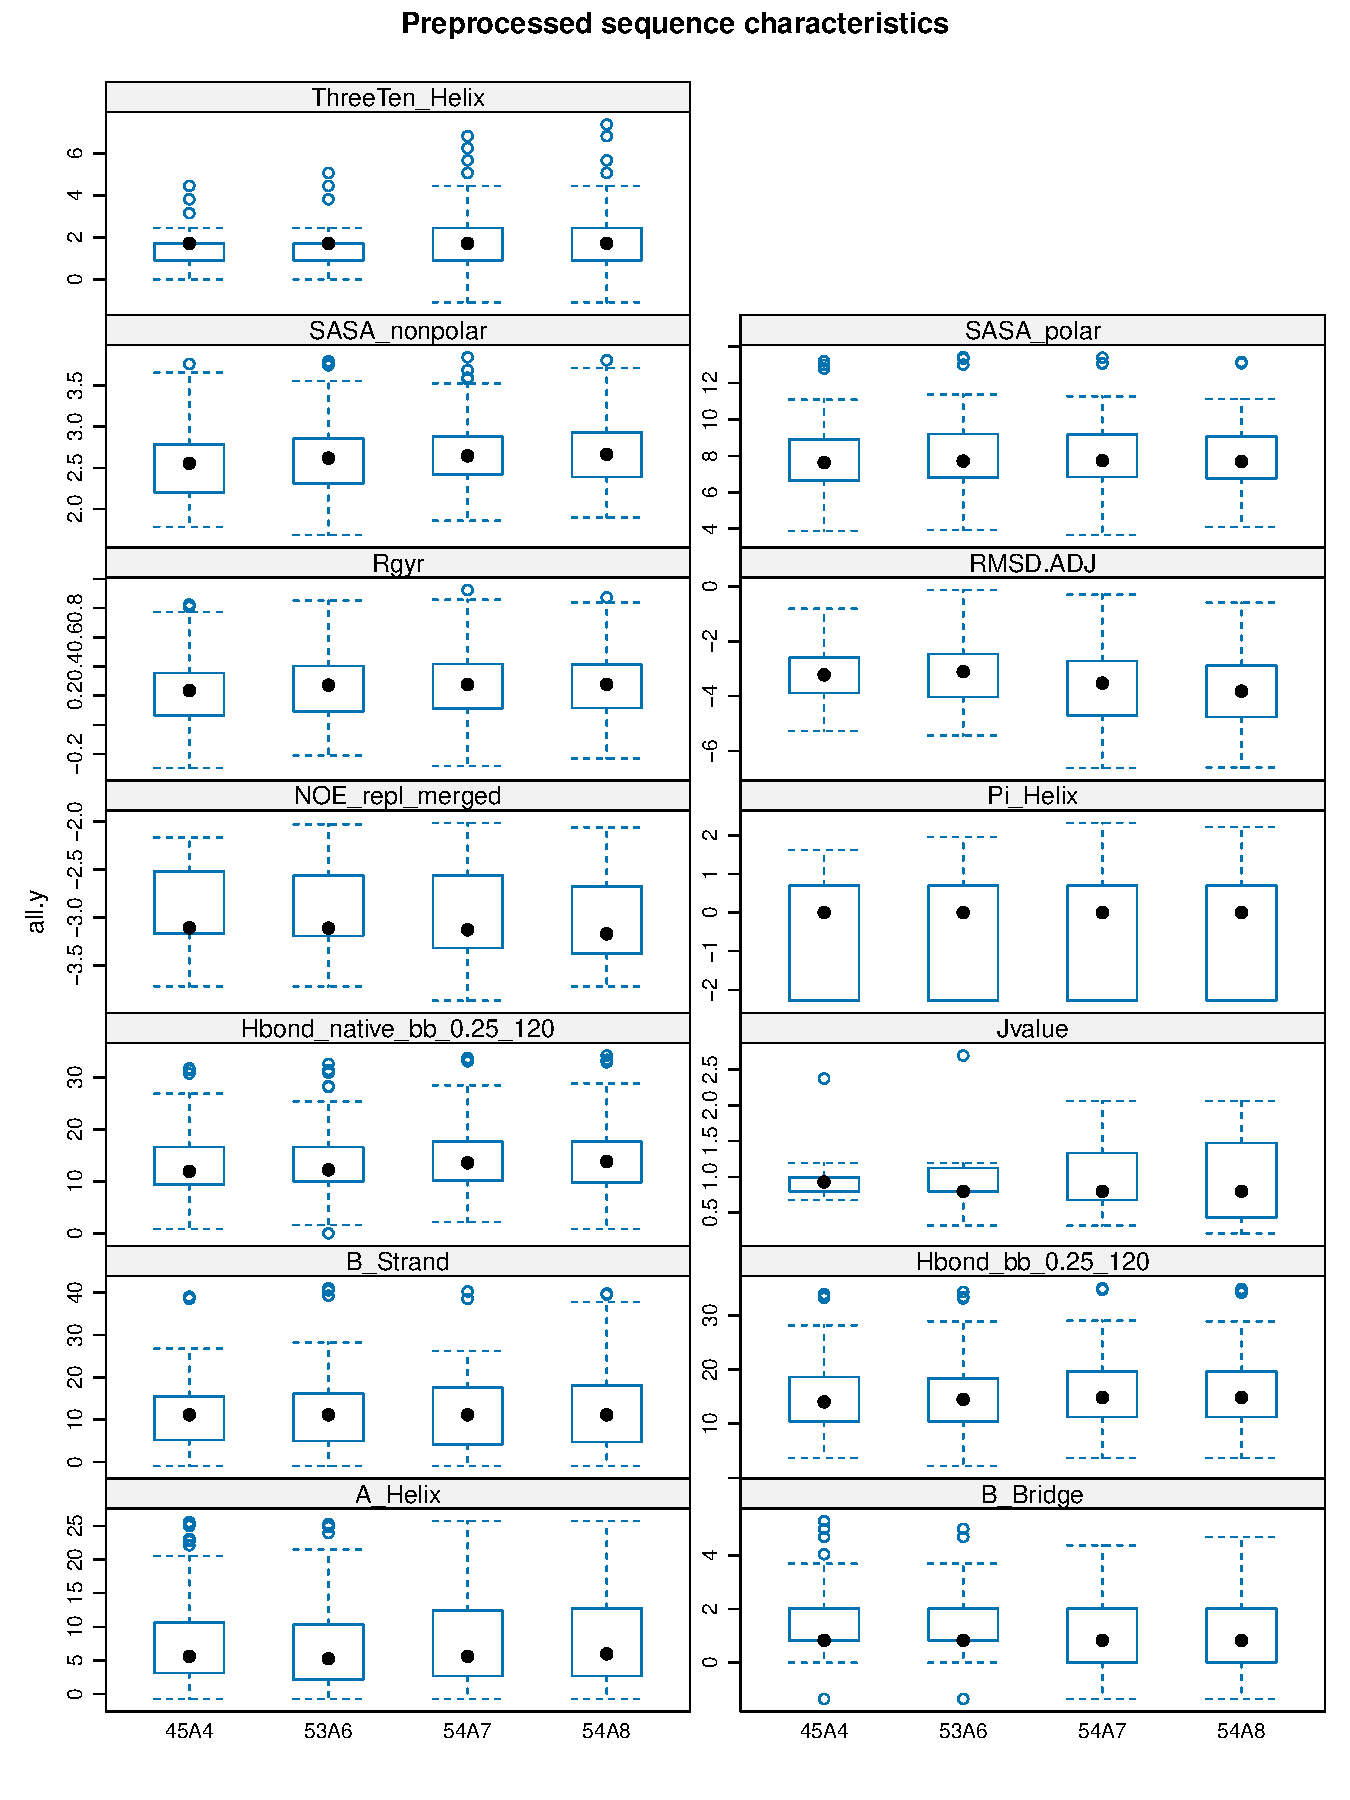
\includegraphics[width=\maxwidth]{figure/bp-chunk-1} 
\end{knitrout}

\subsection{MANOVA and multivariate multilevel analysis}
\begin{knitrout}
\definecolor{shadecolor}{rgb}{0.969, 0.969, 0.969}\color{fgcolor}\begin{kframe}
\begin{verbatim}
##           Model  df      AIC      BIC    logLik   Test  L.Ratio p-value
## lme.fit.n     1 195 5768.429 7080.093 -2689.215                        
## lme.fit.a     2 234 5206.833 6780.830 -2369.417 1 vs 2 639.5958  <.0001
\end{verbatim}
\end{kframe}
\end{knitrout}

The ANOVA output compares the empty model against the more complex
model which uses ``all.alg'' (representing force field) as
regressor. A strongly increased likelihood and far superior AIC and
BIC of the more complex model provide evidence that ``force field''
has a considerable effect on predicted sequence characteristics.
Leading for the likelihood ratio test to a p-value of $<0.0001$, the
differences are of very high statistical significance. The p-value
reported by the anova function follows common practice in statistics,
where small p-values are usually only reported as ``smaller than a
threshold''. The actual p-value from the likelihood ratio test is
$\mathrm{p-val}=1.088e-109$.
\section{Property and algorithm specific mixed model analysis}
After having concluded by a mixed effects regression analysis that the
multivariate metric vector depends significantly on force field, we
will now perform a more detailed analysis. We will to this end rely on
two analyses which assess within metric. 
\begin{enumerate}
\item by a likelihood ratio test whether adding force field as
  regressor leads to significant improvements over the empty (null)
  model.
\item by formulating all ten pairwise contrasts, subsequent
  significance analysis and multiple testing correction whether
  differences between two force fields are statistically significant.
\end{enumerate}
The first stage of this fine grained analysis provides us thus with
twelve p-values which result from the per metric likelihood ratio
tests 1). The second stage of this analysis in 2) provides us across
all metrics and pairwise contrasts with $80$ p-values which assess
whether the respective pair of force fields leads for a particular
metric to significantly different expectations. To control the overall
false positive rate, we adjust the p-values with the Benjamini \&
Yekutieli FDR (BY) for multiple testing.

\begin{knitrout}
\definecolor{shadecolor}{rgb}{0.969, 0.969, 0.969}\color{fgcolor}\begin{kframe}
\begin{verbatim}
## nr pairs: 78
## Order in all.pairs and all.rw.pairs match in:  0  % cases.
## Order in all.pairs and all.dyt.pairs match in:  100  % cases.
## Properties     : A_Helix B_Bridge B_Strand Hbond_bb_0.25_120 Hbond_native_bb_0.25_120 Jvalue NOE_repl_merged Pi_Helix Rgyr RMSD.ADJ SASA_nonpolar SASA_polar ThreeTen_Helix
## Raw p-values   : 1.900596e-06 0.00622542 9.639084e-15 2.188943e-31 5.113798e-29 0.4009499 0.287061 0.2349878 1.117707e-25 5.460412e-11 9.341772e-13 1.120728e-40 0.004307733
## BH adjusted    : 3.088469e-06 0.008093046 2.506162e-14 1.422813e-30 2.215979e-28 0.4009499 0.3109828 0.2777128 3.632549e-25 1.014076e-10 2.024051e-12 1.456947e-39 0.006222282
## BY adjusted    : 9.821744e-06 0.02573697 7.96993e-14 4.524735e-30 7.04711e-28 1 0.9889668 0.8831639 1.155199e-24 3.224899e-10 6.436751e-12 4.633285e-39 0.01978769
\end{verbatim}
\end{kframe}
\end{knitrout}

\subsection{Significance of metric specific likelihood ratio tests}
% kable_styling(latex_options = c("hold_position", "striped", "scale_down")) %>% 


\begin{center}
\begin{table}[!h]

\caption{\label{tab:unnamed-chunk-18}Significance of dependency of univariate metric values on force field}
\centering
\resizebox{\linewidth}{!}{
\begin{tabular}[t]{l|l|l}
\hline
metric & raw.pval & BY.adj\\
\hline
\cellcolor{gray!6}{A\_Helix} & \cellcolor{gray!6}{1.90e-06 (***)} & \cellcolor{gray!6}{9.82e-06 (***)}\\
\hline
B\_Bridge & 6.23e-03  (**) & 2.57e-02   (*)\\
\hline
\cellcolor{gray!6}{B\_Strand} & \cellcolor{gray!6}{9.64e-15 (***)} & \cellcolor{gray!6}{7.97e-14 (***)}\\
\hline
Hbond\_bb\_0.25\_120 & 2.19e-31 (***) & 4.52e-30 (***)\\
\hline
\cellcolor{gray!6}{Hbond\_native\_bb\_0.25\_120} & \cellcolor{gray!6}{5.11e-29 (***)} & \cellcolor{gray!6}{7.05e-28 (***)}\\
\hline
Jvalue & 4.01e-01   ( ) & 1.00e+00   ( )\\
\hline
\cellcolor{gray!6}{NOE\_repl\_merged} & \cellcolor{gray!6}{2.87e-01   ( )} & \cellcolor{gray!6}{9.89e-01   ( )}\\
\hline
Pi\_Helix & 2.35e-01   ( ) & 8.83e-01   ( )\\
\hline
\cellcolor{gray!6}{Rgyr} & \cellcolor{gray!6}{1.12e-25 (***)} & \cellcolor{gray!6}{1.16e-24 (***)}\\
\hline
RMSD.ADJ & 5.46e-11 (***) & 3.22e-10 (***)\\
\hline
\cellcolor{gray!6}{SASA\_nonpolar} & \cellcolor{gray!6}{9.34e-13 (***)} & \cellcolor{gray!6}{6.44e-12 (***)}\\
\hline
SASA\_polar & 1.12e-40 (***) & 4.63e-39 (***)\\
\hline
\cellcolor{gray!6}{ThreeTen\_Helix} & \cellcolor{gray!6}{4.31e-03  (**)} & \cellcolor{gray!6}{1.98e-02   (*)}\\
\hline
\multicolumn{3}{l}{\textsuperscript{a} metric: name of analysed metric; raw.pval: raw p-vale assessing dependencies of metric values on force field for significance; BY.adj: Benjamini \&}\\
\multicolumn{3}{l}{Yekutieli adjusted raw p-values.}\\
\end{tabular}}
\end{table}


\end{center}

By analyzing the results table we conclude that except for the
Pi\_Helix counts, Jvalue and NOE, all other metrics depend
significantly on force field. The adjustment changes significance
levels but does not change our assessment regarding significance.
\subsection{Pairwise comparisons of force fields within metric}



The rows in the subsequent table denote certain binary contrasts. The
table columns contain information about the expected value of the
contrast and the standard error (a $95\%$ confidence interval).  The
Benjamini \& Yekutieli adjusted significance levels assess whether the 
respective metric (transformed values as illustrated in the box plots)

%\begin{tiny}
  %% the following makes the column header diagonal
  %% we also use a table footnote
% kable_styling(latex_options = c("hold_position", "striped", "scale_down")) %>%
%  row_spec(0, angle = 65) %>% 
\begin{center}
\begin{table}[!h]

\caption{\label{tab:unnamed-chunk-19}Binary contrasts between force fields\textsuperscript{a}}
\centering
\resizebox{\linewidth}{!}{
\begin{tabular}[t]{lccccccccccccc}
\toprule
\rotatebox{65}{ } & \rotatebox{65}{A\_Helix} & \rotatebox{65}{B\_Bridge} & \rotatebox{65}{B\_Strand} & \rotatebox{65}{Hbond\_bb\_0.25\_120} & \rotatebox{65}{Hbond\_native\_bb\_0.25\_120} & \rotatebox{65}{Jvalue} & \rotatebox{65}{NOE\_repl\_merged} & \rotatebox{65}{Pi\_Helix} & \rotatebox{65}{Rgyr} & \rotatebox{65}{RMSD.ADJ} & \rotatebox{65}{SASA\_nonpolar} & \rotatebox{65}{SASA\_polar} & \rotatebox{65}{ThreeTen\_Helix}\\
\midrule
\cellcolor{gray!6}{45A4 - 53A6} & \cellcolor{gray!6}{0.36 (***)} & \cellcolor{gray!6}{0.09   ( )} & \cellcolor{gray!6}{-0.13   ( )} & \cellcolor{gray!6}{0.03   ( )} & \cellcolor{gray!6}{-0.31  (**)} & \cellcolor{gray!6}{0.02   ( )} & \cellcolor{gray!6}{-0.05   ( )} & \cellcolor{gray!6}{-0.06   ( )} & \cellcolor{gray!6}{-0.03 (***)} & \cellcolor{gray!6}{-0.07   ( )} & \cellcolor{gray!6}{-0.07 (***)} & \cellcolor{gray!6}{-0.19 (***)} & \cellcolor{gray!6}{0.08   ( )}\\
45A4 - 54A7 & 0.00   ( ) & 0.16   (*) & 0.46 (***) & -0.50 (***) & -0.75 (***) & 0.11   ( ) & -0.02   ( ) & 0.12   ( ) & -0.02 (***) & 0.32  (**) & -0.08 (***) & -0.16 (***) & -0.20   ( )\\
\cellcolor{gray!6}{45A4 - 54A8} & \cellcolor{gray!6}{-0.07   ( )} & \cellcolor{gray!6}{0.18   (*)} & \cellcolor{gray!6}{0.45 (***)} & \cellcolor{gray!6}{-0.56 (***)} & \cellcolor{gray!6}{-0.89 (***)} & \cellcolor{gray!6}{0.13   ( )} & \cellcolor{gray!6}{0.03   ( )} & \cellcolor{gray!6}{0.16   ( )} & \cellcolor{gray!6}{-0.02 (***)} & \cellcolor{gray!6}{0.45 (***)} & \cellcolor{gray!6}{-0.07 (***)} & \cellcolor{gray!6}{-0.10 (***)} & \cellcolor{gray!6}{-0.10   ( )}\\
53A6 - 54A7 & -0.36 (***) & 0.07   ( ) & 0.59 (***) & -0.53 (***) & -0.44 (***) & 0.09   ( ) & 0.03   ( ) & 0.17   ( ) & 0.00   ( ) & 0.39 (***) & -0.00   ( ) & 0.02   ( ) & -0.28  (**)\\
\cellcolor{gray!6}{53A6 - 54A8} & \cellcolor{gray!6}{-0.43 (***)} & \cellcolor{gray!6}{0.09   ( )} & \cellcolor{gray!6}{0.58 (***)} & \cellcolor{gray!6}{-0.59 (***)} & \cellcolor{gray!6}{-0.58 (***)} & \cellcolor{gray!6}{0.11   ( )} & \cellcolor{gray!6}{0.08   ( )} & \cellcolor{gray!6}{0.21   ( )} & \cellcolor{gray!6}{0.00   ( )} & \cellcolor{gray!6}{0.52 (***)} & \cellcolor{gray!6}{0.00   ( )} & \cellcolor{gray!6}{0.09 (***)} & \cellcolor{gray!6}{-0.18   ( )}\\
\addlinespace
54A7 - 54A8 & -0.07   ( ) & 0.02   ( ) & -0.01   ( ) & -0.07   ( ) & -0.14   ( ) & 0.02   ( ) & 0.05   ( ) & 0.04   ( ) & 0.00   ( ) & 0.13   ( ) & 0.00   ( ) & 0.07 (***) & 0.10   ( )\\
\bottomrule
\multicolumn{14}{l}{\textsuperscript{a} Metrics are represented as expected value of the contrast ± standard error (95\% confidence) and an indication of significance with (***) → p-value <0.001, (**) → p-value <0.01, (*) → p-value <0.05 and (.) → p-value <0.1. The p-values are adjusted for multiple testing using the Benjamini \& Yekutieli FDR correction.}\\
\end{tabular}}
\end{table}


\end{center}
%\end{tiny}
\clearpage %% push out fload tables
\subsection{Pairwise assessments of simulation derived values}
\bf{Table S3:} Pairwise differences of protein characteristics between
force fields. Metrics are represented as expected value of the
contrast $\pm$ standard error ($95\%$ confidence) and an indication of
significance with (***) $\rightarrow$ p-value $< 0.001$, (**)
$\rightarrow$ p-value $<0.01$, (*) $\rightarrow$ p-value $<0.05$ and
(.)  $\rightarrow$ p-value $<0.1$. Combinations of contrasts between
force fields and metrics which we find significant are highlighted in
blue.
\begin{center}

\begin{longtable}[t]{lccccc}
\caption{\label{tab:unnamed-chunk-19}Binary contrasts of protein characteristics}\\
\toprule
  & contrast & metric & value & rawval & significance\\
\midrule
\cellcolor{gray!6}{1} & \cellcolor{gray!6}{\textcolor{blue}{45A4 - 53A6}} & \cellcolor{gray!6}{\textcolor{blue}{A\_Helix}} & \cellcolor{gray!6}{\textcolor{blue}{0.36 ± 0.09}} & \cellcolor{gray!6}{\textcolor{blue}{1.26 ± 0.30}} & \cellcolor{gray!6}{\textcolor{black}{(***)}}\\
7 & \textcolor{black}{45A4 - 53A6} & \textcolor{black}{B\_Bridge} & \textcolor{black}{0.09 ± 0.06} & \textcolor{black}{0.18 ± 0.09} & \textcolor{black}{( )}\\
\cellcolor{gray!6}{13} & \cellcolor{gray!6}{\textcolor{black}{45A4 - 53A6}} & \cellcolor{gray!6}{\textcolor{black}{B\_Strand}} & \cellcolor{gray!6}{\textcolor{black}{-0.13 ± 0.09}} & \cellcolor{gray!6}{\textcolor{black}{-0.43 ± 0.21}} & \cellcolor{gray!6}{\textcolor{black}{( )}}\\
19 & \textcolor{black}{45A4 - 53A6} & \textcolor{black}{Hbond\_bb\_0.25\_120} & \textcolor{black}{0.03 ± 0.06} & \textcolor{black}{0.13 ± 0.29} & \textcolor{black}{( )}\\
\cellcolor{gray!6}{25} & \cellcolor{gray!6}{\textcolor{blue}{45A4 - 53A6}} & \cellcolor{gray!6}{\textcolor{blue}{Hbond\_native\_bb\_0.25\_120}} & \cellcolor{gray!6}{\textcolor{blue}{-0.31 ± 0.08}} & \cellcolor{gray!6}{\textcolor{blue}{-1.26 ± 0.35}} & \cellcolor{gray!6}{\textcolor{black}{(**)}}\\
31 & \textcolor{black}{45A4 - 53A6} & \textcolor{black}{Jvalue} & \textcolor{black}{0.02 ± 0.09} & \textcolor{black}{0.03 ± 0.07} & \textcolor{black}{( )}\\
\cellcolor{gray!6}{37} & \cellcolor{gray!6}{\textcolor{black}{45A4 - 53A6}} & \cellcolor{gray!6}{\textcolor{black}{NOE\_repl\_merged}} & \cellcolor{gray!6}{\textcolor{black}{-0.05 ± 0.05}} & \cellcolor{gray!6}{\textcolor{black}{-0.01 ± 0.00}} & \cellcolor{gray!6}{\textcolor{black}{( )}}\\
43 & \textcolor{black}{45A4 - 53A6} & \textcolor{black}{Pi\_Helix} & \textcolor{black}{-0.06 ± 0.12} & \textcolor{black}{-0.09 ± 0.13} & \textcolor{black}{( )}\\
\cellcolor{gray!6}{49} & \cellcolor{gray!6}{\textcolor{blue}{45A4 - 53A6}} & \cellcolor{gray!6}{\textcolor{blue}{Rgyr}} & \cellcolor{gray!6}{\textcolor{blue}{-0.03 ± 0.00}} & \cellcolor{gray!6}{\textcolor{blue}{-0.03 ± 0.00}} & \cellcolor{gray!6}{\textcolor{black}{(***)}}\\
55 & \textcolor{black}{45A4 - 53A6} & \textcolor{black}{RMSD.ADJ} & \textcolor{black}{-0.07 ± 0.09} & \textcolor{black}{-0.02 ± 0.01} & \textcolor{black}{( )}\\
\cellcolor{gray!6}{61} & \cellcolor{gray!6}{\textcolor{blue}{45A4 - 53A6}} & \cellcolor{gray!6}{\textcolor{blue}{SASA\_nonpolar}} & \cellcolor{gray!6}{\textcolor{blue}{-0.07 ± 0.01}} & \cellcolor{gray!6}{\textcolor{blue}{-0.54 ± 0.09}} & \cellcolor{gray!6}{\textcolor{black}{(***)}}\\
67 & \textcolor{blue}{45A4 - 53A6} & \textcolor{blue}{SASA\_polar} & \textcolor{blue}{-0.19 ± 0.01} & \textcolor{blue}{-1.56 ± 0.12} & \textcolor{black}{(***)}\\
\cellcolor{gray!6}{73} & \cellcolor{gray!6}{\textcolor{black}{45A4 - 53A6}} & \cellcolor{gray!6}{\textcolor{black}{ThreeTen\_Helix}} & \cellcolor{gray!6}{\textcolor{black}{0.08 ± 0.08}} & \cellcolor{gray!6}{\textcolor{black}{0.10 ± 0.11}} & \cellcolor{gray!6}{\textcolor{black}{( )}}\\
2 & \textcolor{black}{45A4 - 54A7} & \textcolor{black}{A\_Helix} & \textcolor{black}{0.00 ± 0.08} & \textcolor{black}{-0.42 ± 0.29} & \textcolor{black}{( )}\\
\cellcolor{gray!6}{8} & \cellcolor{gray!6}{\textcolor{blue}{45A4 - 54A7}} & \cellcolor{gray!6}{\textcolor{blue}{B\_Bridge}} & \cellcolor{gray!6}{\textcolor{blue}{0.16 ± 0.06}} & \cellcolor{gray!6}{\textcolor{blue}{0.20 ± 0.08}} & \cellcolor{gray!6}{\textcolor{black}{(*)}}\\
14 & \textcolor{blue}{45A4 - 54A7} & \textcolor{blue}{B\_Strand} & \textcolor{blue}{0.46 ± 0.08} & \textcolor{blue}{0.94 ± 0.20} & \textcolor{black}{(***)}\\
\cellcolor{gray!6}{20} & \cellcolor{gray!6}{\textcolor{blue}{45A4 - 54A7}} & \cellcolor{gray!6}{\textcolor{blue}{Hbond\_bb\_0.25\_120}} & \cellcolor{gray!6}{\textcolor{blue}{-0.50 ± 0.06}} & \cellcolor{gray!6}{\textcolor{blue}{-2.46 ± 0.28}} & \cellcolor{gray!6}{\textcolor{black}{(***)}}\\
26 & \textcolor{blue}{45A4 - 54A7} & \textcolor{blue}{Hbond\_native\_bb\_0.25\_120} & \textcolor{blue}{-0.75 ± 0.08} & \textcolor{blue}{-3.12 ± 0.34} & \textcolor{black}{(***)}\\
\cellcolor{gray!6}{32} & \cellcolor{gray!6}{\textcolor{black}{45A4 - 54A7}} & \cellcolor{gray!6}{\textcolor{black}{Jvalue}} & \cellcolor{gray!6}{\textcolor{black}{0.11 ± 0.09}} & \cellcolor{gray!6}{\textcolor{black}{0.09 ± 0.07}} & \cellcolor{gray!6}{\textcolor{black}{( )}}\\
38 & \textcolor{black}{45A4 - 54A7} & \textcolor{black}{NOE\_repl\_merged} & \textcolor{black}{-0.02 ± 0.05} & \textcolor{black}{-0.00 ± 0.00} & \textcolor{black}{( )}\\
\cellcolor{gray!6}{44} & \cellcolor{gray!6}{\textcolor{black}{45A4 - 54A7}} & \cellcolor{gray!6}{\textcolor{black}{Pi\_Helix}} & \cellcolor{gray!6}{\textcolor{black}{0.12 ± 0.11}} & \cellcolor{gray!6}{\textcolor{black}{0.13 ± 0.13}} & \cellcolor{gray!6}{\textcolor{black}{( )}}\\
50 & \textcolor{blue}{45A4 - 54A7} & \textcolor{blue}{Rgyr} & \textcolor{blue}{-0.02 ± 0.00} & \textcolor{blue}{-0.03 ± 0.00} & \textcolor{black}{(***)}\\
\cellcolor{gray!6}{56} & \cellcolor{gray!6}{\textcolor{blue}{45A4 - 54A7}} & \cellcolor{gray!6}{\textcolor{blue}{RMSD.ADJ}} & \cellcolor{gray!6}{\textcolor{blue}{0.32 ± 0.08}} & \cellcolor{gray!6}{\textcolor{blue}{0.01 ± 0.01}} & \cellcolor{gray!6}{\textcolor{black}{(**)}}\\
62 & \textcolor{blue}{45A4 - 54A7} & \textcolor{blue}{SASA\_nonpolar} & \textcolor{blue}{-0.08 ± 0.01} & \textcolor{blue}{-0.53 ± 0.09} & \textcolor{black}{(***)}\\
\cellcolor{gray!6}{68} & \cellcolor{gray!6}{\textcolor{blue}{45A4 - 54A7}} & \cellcolor{gray!6}{\textcolor{blue}{SASA\_polar}} & \cellcolor{gray!6}{\textcolor{blue}{-0.16 ± 0.01}} & \cellcolor{gray!6}{\textcolor{blue}{-1.35 ± 0.12}} & \cellcolor{gray!6}{\textcolor{black}{(***)}}\\
74 & \textcolor{black}{45A4 - 54A7} & \textcolor{black}{ThreeTen\_Helix} & \textcolor{black}{-0.20 ± 0.08} & \textcolor{black}{-0.29 ± 0.11} & \textcolor{black}{( )}\\
\cellcolor{gray!6}{3} & \cellcolor{gray!6}{\textcolor{black}{45A4 - 54A8}} & \cellcolor{gray!6}{\textcolor{black}{A\_Helix}} & \cellcolor{gray!6}{\textcolor{black}{-0.07 ± 0.08}} & \cellcolor{gray!6}{\textcolor{black}{-0.67 ± 0.29}} & \cellcolor{gray!6}{\textcolor{black}{( )}}\\
9 & \textcolor{blue}{45A4 - 54A8} & \textcolor{blue}{B\_Bridge} & \textcolor{blue}{0.18 ± 0.06} & \textcolor{blue}{0.22 ± 0.08} & \textcolor{black}{(*)}\\
\cellcolor{gray!6}{15} & \cellcolor{gray!6}{\textcolor{blue}{45A4 - 54A8}} & \cellcolor{gray!6}{\textcolor{blue}{B\_Strand}} & \cellcolor{gray!6}{\textcolor{blue}{0.45 ± 0.08}} & \cellcolor{gray!6}{\textcolor{blue}{0.88 ± 0.20}} & \cellcolor{gray!6}{\textcolor{black}{(***)}}\\
21 & \textcolor{blue}{45A4 - 54A8} & \textcolor{blue}{Hbond\_bb\_0.25\_120} & \textcolor{blue}{-0.56 ± 0.06} & \textcolor{blue}{-2.75 ± 0.28} & \textcolor{black}{(***)}\\
\cellcolor{gray!6}{27} & \cellcolor{gray!6}{\textcolor{blue}{45A4 - 54A8}} & \cellcolor{gray!6}{\textcolor{blue}{Hbond\_native\_bb\_0.25\_120}} & \cellcolor{gray!6}{\textcolor{blue}{-0.89 ± 0.08}} & \cellcolor{gray!6}{\textcolor{blue}{-3.66 ± 0.34}} & \cellcolor{gray!6}{\textcolor{black}{(***)}}\\
33 & \textcolor{black}{45A4 - 54A8} & \textcolor{black}{Jvalue} & \textcolor{black}{0.13 ± 0.09} & \textcolor{black}{0.11 ± 0.07} & \textcolor{black}{( )}\\
\cellcolor{gray!6}{39} & \cellcolor{gray!6}{\textcolor{black}{45A4 - 54A8}} & \cellcolor{gray!6}{\textcolor{black}{NOE\_repl\_merged}} & \cellcolor{gray!6}{\textcolor{black}{0.03 ± 0.05}} & \cellcolor{gray!6}{\textcolor{black}{-0.00 ± 0.00}} & \cellcolor{gray!6}{\textcolor{black}{( )}}\\
45 & \textcolor{black}{45A4 - 54A8} & \textcolor{black}{Pi\_Helix} & \textcolor{black}{0.16 ± 0.11} & \textcolor{black}{0.21 ± 0.13} & \textcolor{black}{( )}\\
\cellcolor{gray!6}{51} & \cellcolor{gray!6}{\textcolor{blue}{45A4 - 54A8}} & \cellcolor{gray!6}{\textcolor{blue}{Rgyr}} & \cellcolor{gray!6}{\textcolor{blue}{-0.02 ± 0.00}} & \cellcolor{gray!6}{\textcolor{blue}{-0.02 ± 0.00}} & \cellcolor{gray!6}{\textcolor{black}{(***)}}\\
57 & \textcolor{blue}{45A4 - 54A8} & \textcolor{blue}{RMSD.ADJ} & \textcolor{blue}{0.45 ± 0.08} & \textcolor{blue}{0.02 ± 0.01} & \textcolor{black}{(***)}\\
\cellcolor{gray!6}{63} & \cellcolor{gray!6}{\textcolor{blue}{45A4 - 54A8}} & \cellcolor{gray!6}{\textcolor{blue}{SASA\_nonpolar}} & \cellcolor{gray!6}{\textcolor{blue}{-0.07 ± 0.01}} & \cellcolor{gray!6}{\textcolor{blue}{-0.50 ± 0.09}} & \cellcolor{gray!6}{\textcolor{black}{(***)}}\\
69 & \textcolor{blue}{45A4 - 54A8} & \textcolor{blue}{SASA\_polar} & \textcolor{blue}{-0.10 ± 0.01} & \textcolor{blue}{-0.79 ± 0.12} & \textcolor{black}{(***)}\\
\cellcolor{gray!6}{75} & \cellcolor{gray!6}{\textcolor{black}{45A4 - 54A8}} & \cellcolor{gray!6}{\textcolor{black}{ThreeTen\_Helix}} & \cellcolor{gray!6}{\textcolor{black}{-0.10 ± 0.08}} & \cellcolor{gray!6}{\textcolor{black}{-0.17 ± 0.11}} & \cellcolor{gray!6}{\textcolor{black}{( )}}\\
4 & \textcolor{blue}{53A6 - 54A7} & \textcolor{blue}{A\_Helix} & \textcolor{blue}{-0.36 ± 0.08} & \textcolor{blue}{-1.68 ± 0.29} & \textcolor{black}{(***)}\\
\cellcolor{gray!6}{10} & \cellcolor{gray!6}{\textcolor{black}{53A6 - 54A7}} & \cellcolor{gray!6}{\textcolor{black}{B\_Bridge}} & \cellcolor{gray!6}{\textcolor{black}{0.07 ± 0.06}} & \cellcolor{gray!6}{\textcolor{black}{0.01 ± 0.08}} & \cellcolor{gray!6}{\textcolor{black}{( )}}\\
16 & \textcolor{blue}{53A6 - 54A7} & \textcolor{blue}{B\_Strand} & \textcolor{blue}{0.59 ± 0.08} & \textcolor{blue}{1.38 ± 0.20} & \textcolor{black}{(***)}\\
\cellcolor{gray!6}{22} & \cellcolor{gray!6}{\textcolor{blue}{53A6 - 54A7}} & \cellcolor{gray!6}{\textcolor{blue}{Hbond\_bb\_0.25\_120}} & \cellcolor{gray!6}{\textcolor{blue}{-0.53 ± 0.06}} & \cellcolor{gray!6}{\textcolor{blue}{-2.58 ± 0.28}} & \cellcolor{gray!6}{\textcolor{black}{(***)}}\\
28 & \textcolor{blue}{53A6 - 54A7} & \textcolor{blue}{Hbond\_native\_bb\_0.25\_120} & \textcolor{blue}{-0.44 ± 0.08} & \textcolor{blue}{-1.86 ± 0.34} & \textcolor{black}{(***)}\\
\cellcolor{gray!6}{34} & \cellcolor{gray!6}{\textcolor{black}{53A6 - 54A7}} & \cellcolor{gray!6}{\textcolor{black}{Jvalue}} & \cellcolor{gray!6}{\textcolor{black}{0.09 ± 0.09}} & \cellcolor{gray!6}{\textcolor{black}{0.06 ± 0.07}} & \cellcolor{gray!6}{\textcolor{black}{( )}}\\
40 & \textcolor{black}{53A6 - 54A7} & \textcolor{black}{NOE\_repl\_merged} & \textcolor{black}{0.03 ± 0.04} & \textcolor{black}{0.00 ± 0.00} & \textcolor{black}{( )}\\
\cellcolor{gray!6}{46} & \cellcolor{gray!6}{\textcolor{black}{53A6 - 54A7}} & \cellcolor{gray!6}{\textcolor{black}{Pi\_Helix}} & \cellcolor{gray!6}{\textcolor{black}{0.17 ± 0.11}} & \cellcolor{gray!6}{\textcolor{black}{0.22 ± 0.13}} & \cellcolor{gray!6}{\textcolor{black}{( )}}\\
52 & \textcolor{black}{53A6 - 54A7} & \textcolor{black}{Rgyr} & \textcolor{black}{0.00 ± 0.00} & \textcolor{black}{0.00 ± 0.00} & \textcolor{black}{( )}\\
\cellcolor{gray!6}{58} & \cellcolor{gray!6}{\textcolor{blue}{53A6 - 54A7}} & \cellcolor{gray!6}{\textcolor{blue}{RMSD.ADJ}} & \cellcolor{gray!6}{\textcolor{blue}{0.39 ± 0.08}} & \cellcolor{gray!6}{\textcolor{blue}{0.03 ± 0.01}} & \cellcolor{gray!6}{\textcolor{black}{(***)}}\\
64 & \textcolor{black}{53A6 - 54A7} & \textcolor{black}{SASA\_nonpolar} & \textcolor{black}{-0.00 ± 0.01} & \textcolor{black}{0.01 ± 0.09} & \textcolor{black}{( )}\\
\cellcolor{gray!6}{70} & \cellcolor{gray!6}{\textcolor{black}{53A6 - 54A7}} & \cellcolor{gray!6}{\textcolor{black}{SASA\_polar}} & \cellcolor{gray!6}{\textcolor{black}{0.02 ± 0.01}} & \cellcolor{gray!6}{\textcolor{black}{0.22 ± 0.12}} & \cellcolor{gray!6}{\textcolor{black}{( )}}\\
76 & \textcolor{blue}{53A6 - 54A7} & \textcolor{blue}{ThreeTen\_Helix} & \textcolor{blue}{-0.28 ± 0.08} & \textcolor{blue}{-0.39 ± 0.11} & \textcolor{black}{(**)}\\
\cellcolor{gray!6}{5} & \cellcolor{gray!6}{\textcolor{blue}{53A6 - 54A8}} & \cellcolor{gray!6}{\textcolor{blue}{A\_Helix}} & \cellcolor{gray!6}{\textcolor{blue}{-0.43 ± 0.08}} & \cellcolor{gray!6}{\textcolor{blue}{-1.94 ± 0.29}} & \cellcolor{gray!6}{\textcolor{black}{(***)}}\\
11 & \textcolor{black}{53A6 - 54A8} & \textcolor{black}{B\_Bridge} & \textcolor{black}{0.09 ± 0.06} & \textcolor{black}{0.04 ± 0.08} & \textcolor{black}{( )}\\
\cellcolor{gray!6}{17} & \cellcolor{gray!6}{\textcolor{blue}{53A6 - 54A8}} & \cellcolor{gray!6}{\textcolor{blue}{B\_Strand}} & \cellcolor{gray!6}{\textcolor{blue}{0.58 ± 0.08}} & \cellcolor{gray!6}{\textcolor{blue}{1.31 ± 0.20}} & \cellcolor{gray!6}{\textcolor{black}{(***)}}\\
23 & \textcolor{blue}{53A6 - 54A8} & \textcolor{blue}{Hbond\_bb\_0.25\_120} & \textcolor{blue}{-0.59 ± 0.06} & \textcolor{blue}{-2.88 ± 0.28} & \textcolor{black}{(***)}\\
\cellcolor{gray!6}{29} & \cellcolor{gray!6}{\textcolor{blue}{53A6 - 54A8}} & \cellcolor{gray!6}{\textcolor{blue}{Hbond\_native\_bb\_0.25\_120}} & \cellcolor{gray!6}{\textcolor{blue}{-0.58 ± 0.08}} & \cellcolor{gray!6}{\textcolor{blue}{-2.40 ± 0.34}} & \cellcolor{gray!6}{\textcolor{black}{(***)}}\\
35 & \textcolor{black}{53A6 - 54A8} & \textcolor{black}{Jvalue} & \textcolor{black}{0.11 ± 0.09} & \textcolor{black}{0.08 ± 0.07} & \textcolor{black}{( )}\\
\cellcolor{gray!6}{41} & \cellcolor{gray!6}{\textcolor{black}{53A6 - 54A8}} & \cellcolor{gray!6}{\textcolor{black}{NOE\_repl\_merged}} & \cellcolor{gray!6}{\textcolor{black}{0.08 ± 0.04}} & \cellcolor{gray!6}{\textcolor{black}{0.00 ± 0.00}} & \cellcolor{gray!6}{\textcolor{black}{( )}}\\
47 & \textcolor{black}{53A6 - 54A8} & \textcolor{black}{Pi\_Helix} & \textcolor{black}{0.21 ± 0.11} & \textcolor{black}{0.30 ± 0.13} & \textcolor{black}{( )}\\
\cellcolor{gray!6}{53} & \cellcolor{gray!6}{\textcolor{black}{53A6 - 54A8}} & \cellcolor{gray!6}{\textcolor{black}{Rgyr}} & \cellcolor{gray!6}{\textcolor{black}{0.00 ± 0.00}} & \cellcolor{gray!6}{\textcolor{black}{0.01 ± 0.00}} & \cellcolor{gray!6}{\textcolor{black}{( )}}\\
59 & \textcolor{blue}{53A6 - 54A8} & \textcolor{blue}{RMSD.ADJ} & \textcolor{blue}{0.52 ± 0.08} & \textcolor{blue}{0.04 ± 0.01} & \textcolor{black}{(***)}\\
\cellcolor{gray!6}{65} & \cellcolor{gray!6}{\textcolor{black}{53A6 - 54A8}} & \cellcolor{gray!6}{\textcolor{black}{SASA\_nonpolar}} & \cellcolor{gray!6}{\textcolor{black}{0.00 ± 0.01}} & \cellcolor{gray!6}{\textcolor{black}{0.04 ± 0.09}} & \cellcolor{gray!6}{\textcolor{black}{( )}}\\
71 & \textcolor{blue}{53A6 - 54A8} & \textcolor{blue}{SASA\_polar} & \textcolor{blue}{0.09 ± 0.01} & \textcolor{blue}{0.78 ± 0.12} & \textcolor{black}{(***)}\\
\cellcolor{gray!6}{77} & \cellcolor{gray!6}{\textcolor{black}{53A6 - 54A8}} & \cellcolor{gray!6}{\textcolor{black}{ThreeTen\_Helix}} & \cellcolor{gray!6}{\textcolor{black}{-0.18 ± 0.08}} & \cellcolor{gray!6}{\textcolor{black}{-0.27 ± 0.11}} & \cellcolor{gray!6}{\textcolor{black}{( )}}\\
6 & \textcolor{black}{54A7 - 54A8} & \textcolor{black}{A\_Helix} & \textcolor{black}{-0.07 ± 0.08} & \textcolor{black}{-0.26 ± 0.26} & \textcolor{black}{( )}\\
\cellcolor{gray!6}{12} & \cellcolor{gray!6}{\textcolor{black}{54A7 - 54A8}} & \cellcolor{gray!6}{\textcolor{black}{B\_Bridge}} & \cellcolor{gray!6}{\textcolor{black}{0.02 ± 0.05}} & \cellcolor{gray!6}{\textcolor{black}{0.02 ± 0.08}} & \cellcolor{gray!6}{\textcolor{black}{( )}}\\
18 & \textcolor{black}{54A7 - 54A8} & \textcolor{black}{B\_Strand} & \textcolor{black}{-0.01 ± 0.08} & \textcolor{black}{-0.06 ± 0.18} & \textcolor{black}{( )}\\
\cellcolor{gray!6}{24} & \cellcolor{gray!6}{\textcolor{black}{54A7 - 54A8}} & \cellcolor{gray!6}{\textcolor{black}{Hbond\_bb\_0.25\_120}} & \cellcolor{gray!6}{\textcolor{black}{-0.07 ± 0.05}} & \cellcolor{gray!6}{\textcolor{black}{-0.29 ± 0.26}} & \cellcolor{gray!6}{\textcolor{black}{( )}}\\
30 & \textcolor{black}{54A7 - 54A8} & \textcolor{black}{Hbond\_native\_bb\_0.25\_120} & \textcolor{black}{-0.14 ± 0.07} & \textcolor{black}{-0.54 ± 0.30} & \textcolor{black}{( )}\\
\cellcolor{gray!6}{36} & \cellcolor{gray!6}{\textcolor{black}{54A7 - 54A8}} & \cellcolor{gray!6}{\textcolor{black}{Jvalue}} & \cellcolor{gray!6}{\textcolor{black}{0.02 ± 0.09}} & \cellcolor{gray!6}{\textcolor{black}{0.03 ± 0.07}} & \cellcolor{gray!6}{\textcolor{black}{( )}}\\
42 & \textcolor{black}{54A7 - 54A8} & \textcolor{black}{NOE\_repl\_merged} & \textcolor{black}{0.05 ± 0.04} & \textcolor{black}{0.00 ± 0.00} & \textcolor{black}{( )}\\
\cellcolor{gray!6}{48} & \cellcolor{gray!6}{\textcolor{black}{54A7 - 54A8}} & \cellcolor{gray!6}{\textcolor{black}{Pi\_Helix}} & \cellcolor{gray!6}{\textcolor{black}{0.04 ± 0.10}} & \cellcolor{gray!6}{\textcolor{black}{0.08 ± 0.11}} & \cellcolor{gray!6}{\textcolor{black}{( )}}\\
54 & \textcolor{black}{54A7 - 54A8} & \textcolor{black}{Rgyr} & \textcolor{black}{0.00 ± 0.00} & \textcolor{black}{0.00 ± 0.00} & \textcolor{black}{( )}\\
\cellcolor{gray!6}{60} & \cellcolor{gray!6}{\textcolor{black}{54A7 - 54A8}} & \cellcolor{gray!6}{\textcolor{black}{RMSD.ADJ}} & \cellcolor{gray!6}{\textcolor{black}{0.13 ± 0.07}} & \cellcolor{gray!6}{\textcolor{black}{0.01 ± 0.01}} & \cellcolor{gray!6}{\textcolor{black}{( )}}\\
66 & \textcolor{black}{54A7 - 54A8} & \textcolor{black}{SASA\_nonpolar} & \textcolor{black}{0.00 ± 0.01} & \textcolor{black}{0.03 ± 0.08} & \textcolor{black}{( )}\\
\cellcolor{gray!6}{72} & \cellcolor{gray!6}{\textcolor{blue}{54A7 - 54A8}} & \cellcolor{gray!6}{\textcolor{blue}{SASA\_polar}} & \cellcolor{gray!6}{\textcolor{blue}{0.07 ± 0.01}} & \cellcolor{gray!6}{\textcolor{blue}{0.56 ± 0.10}} & \cellcolor{gray!6}{\textcolor{black}{(***)}}\\
78 & \textcolor{black}{54A7 - 54A8} & \textcolor{black}{ThreeTen\_Helix} & \textcolor{black}{0.10 ± 0.07} & \textcolor{black}{0.12 ± 0.10} & \textcolor{black}{( )}\\
\bottomrule
\end{longtable}


\end{center}
%%>% 
%  add_footnote("Metrics are represented as expected value of the contrast \U00B1 standard error (95% confidence) and an indication of signifi%cance with (***) \U2192 p-value \textless 0.001, (**) \U2192 p-value <0.01, (*) \U2192 p-value <0.05 and (.) \U2192 p-value <0.1. Combination%s of contrasts between force fields and metrics which we find significant are highlighted in blue.")
\subsection{Pairwise assessments of simulation derived differences from crystal structure derived truth}

\bf{Table S4:} Pairwise assessments of the discrepancies of simulation
derived and experimentally validated protein characteristics.
Differences between simulation derived and structure based protein
characteristics are represented as expected value of the contrast
$\pm$ standard error ($95\%$ confidence) and an indication of
significance with (***) $\rightarrow$ p-value $< 0.001$, (**)
$\rightarrow$ p-value $<0.01$, (*) $\rightarrow$ p-value $<0.05$ and
(.)  $\rightarrow$ p-value $<0.1$. Combinations of contrasts between
force fields and metrics which we find significant are highlighted in
blue. To put these results into relation with table S1, we note that
the results reported in table S2 will in general differ in p-vale and
sign and absolute value of the expected contrast value from those in
table S1. The exact same result will however be observed if the
crystal derived ``truth'' is {\it smaller} than the simulation derived
characteristics obtained with both force fields considered. The same
p-value and an expected contrast with identical absolute value and
alternating sign will be observed if the crystal derived ``truth'' is
{\it larger} than the simulation derived characteristics obtained with
both force fields considered.

A positive sign of the expected contrast value indicates that
the force field which enters the contrast positively is closer to the
crystal structure derived value. The alternating signs we observe in
dependence of metric for a particular pair of force fields indicate
that preference depends on the metrics considered. Unequivocal
preferences for a particular force field can thus in general not be
stated from these analyses. 

\begin{center}

\begin{longtable}[t]{lcccc}
\caption{\label{tab:unnamed-chunk-19}Binary contrasts of protein characteristic differences in simulation and measurement}\\
\toprule
  & contrast & metric & value & significance\\
\midrule
\cellcolor{gray!6}{1} & \cellcolor{gray!6}{\textcolor{blue}{45A4 - 53A6}} & \cellcolor{gray!6}{\textcolor{blue}{A\_Helix}} & \cellcolor{gray!6}{\textcolor{blue}{0.36 ± 0.09}} & \cellcolor{gray!6}{\textcolor{black}{(***)}}\\
7 & \textcolor{black}{45A4 - 53A6} & \textcolor{black}{B\_Bridge} & \textcolor{black}{0.09 ± 0.06} & \textcolor{black}{( )}\\
\cellcolor{gray!6}{13} & \cellcolor{gray!6}{\textcolor{black}{45A4 - 53A6}} & \cellcolor{gray!6}{\textcolor{black}{B\_Strand}} & \cellcolor{gray!6}{\textcolor{black}{-0.13 ± 0.09}} & \cellcolor{gray!6}{\textcolor{black}{( )}}\\
19 & \textcolor{black}{45A4 - 53A6} & \textcolor{black}{Hbond\_bb\_0.25\_120} & \textcolor{black}{0.03 ± 0.06} & \textcolor{black}{( )}\\
\cellcolor{gray!6}{25} & \cellcolor{gray!6}{\textcolor{blue}{45A4 - 53A6}} & \cellcolor{gray!6}{\textcolor{blue}{Hbond\_native\_bb\_0.25\_120}} & \cellcolor{gray!6}{\textcolor{blue}{-0.31 ± 0.08}} & \cellcolor{gray!6}{\textcolor{black}{(**)}}\\
31 & \textcolor{black}{45A4 - 53A6} & \textcolor{black}{Jvalue} & \textcolor{black}{0.02 ± 0.09} & \textcolor{black}{( )}\\
\cellcolor{gray!6}{37} & \cellcolor{gray!6}{\textcolor{black}{45A4 - 53A6}} & \cellcolor{gray!6}{\textcolor{black}{NOE\_repl\_merged}} & \cellcolor{gray!6}{\textcolor{black}{-0.05 ± 0.05}} & \cellcolor{gray!6}{\textcolor{black}{( )}}\\
43 & \textcolor{black}{45A4 - 53A6} & \textcolor{black}{Pi\_Helix} & \textcolor{black}{-0.06 ± 0.12} & \textcolor{black}{( )}\\
\cellcolor{gray!6}{49} & \cellcolor{gray!6}{\textcolor{blue}{45A4 - 53A6}} & \cellcolor{gray!6}{\textcolor{blue}{Rgyr}} & \cellcolor{gray!6}{\textcolor{blue}{-0.02 ± 0.00}} & \cellcolor{gray!6}{\textcolor{black}{(***)}}\\
55 & \textcolor{black}{45A4 - 53A6} & \textcolor{black}{RMSD.ADJ} & \textcolor{black}{-0.07 ± 0.09} & \textcolor{black}{( )}\\
\cellcolor{gray!6}{61} & \cellcolor{gray!6}{\textcolor{blue}{45A4 - 53A6}} & \cellcolor{gray!6}{\textcolor{blue}{SASA\_nonpolar}} & \cellcolor{gray!6}{\textcolor{blue}{-0.06 ± 0.01}} & \cellcolor{gray!6}{\textcolor{black}{(***)}}\\
67 & \textcolor{blue}{45A4 - 53A6} & \textcolor{blue}{SASA\_polar} & \textcolor{blue}{-0.13 ± 0.02} & \textcolor{black}{(***)}\\
\cellcolor{gray!6}{73} & \cellcolor{gray!6}{\textcolor{black}{45A4 - 53A6}} & \cellcolor{gray!6}{\textcolor{black}{ThreeTen\_Helix}} & \cellcolor{gray!6}{\textcolor{black}{0.08 ± 0.08}} & \cellcolor{gray!6}{\textcolor{black}{( )}}\\
2 & \textcolor{black}{45A4 - 54A7} & \textcolor{black}{A\_Helix} & \textcolor{black}{0.00 ± 0.08} & \textcolor{black}{( )}\\
\cellcolor{gray!6}{8} & \cellcolor{gray!6}{\textcolor{blue}{45A4 - 54A7}} & \cellcolor{gray!6}{\textcolor{blue}{B\_Bridge}} & \cellcolor{gray!6}{\textcolor{blue}{0.16 ± 0.06}} & \cellcolor{gray!6}{\textcolor{black}{(*)}}\\
14 & \textcolor{blue}{45A4 - 54A7} & \textcolor{blue}{B\_Strand} & \textcolor{blue}{0.47 ± 0.08} & \textcolor{black}{(***)}\\
\cellcolor{gray!6}{20} & \cellcolor{gray!6}{\textcolor{blue}{45A4 - 54A7}} & \cellcolor{gray!6}{\textcolor{blue}{Hbond\_bb\_0.25\_120}} & \cellcolor{gray!6}{\textcolor{blue}{-0.51 ± 0.06}} & \cellcolor{gray!6}{\textcolor{black}{(***)}}\\
26 & \textcolor{blue}{45A4 - 54A7} & \textcolor{blue}{Hbond\_native\_bb\_0.25\_120} & \textcolor{blue}{-0.77 ± 0.08} & \textcolor{black}{(***)}\\
\cellcolor{gray!6}{32} & \cellcolor{gray!6}{\textcolor{black}{45A4 - 54A7}} & \cellcolor{gray!6}{\textcolor{black}{Jvalue}} & \cellcolor{gray!6}{\textcolor{black}{0.12 ± 0.09}} & \cellcolor{gray!6}{\textcolor{black}{( )}}\\
38 & \textcolor{black}{45A4 - 54A7} & \textcolor{black}{NOE\_repl\_merged} & \textcolor{black}{-0.02 ± 0.05} & \textcolor{black}{( )}\\
\cellcolor{gray!6}{44} & \cellcolor{gray!6}{\textcolor{black}{45A4 - 54A7}} & \cellcolor{gray!6}{\textcolor{black}{Pi\_Helix}} & \cellcolor{gray!6}{\textcolor{black}{0.12 ± 0.11}} & \cellcolor{gray!6}{\textcolor{black}{( )}}\\
50 & \textcolor{blue}{45A4 - 54A7} & \textcolor{blue}{Rgyr} & \textcolor{blue}{-0.02 ± 0.00} & \textcolor{black}{(***)}\\
\cellcolor{gray!6}{56} & \cellcolor{gray!6}{\textcolor{blue}{45A4 - 54A7}} & \cellcolor{gray!6}{\textcolor{blue}{RMSD.ADJ}} & \cellcolor{gray!6}{\textcolor{blue}{0.32 ± 0.08}} & \cellcolor{gray!6}{\textcolor{black}{(**)}}\\
62 & \textcolor{blue}{45A4 - 54A7} & \textcolor{blue}{SASA\_nonpolar} & \textcolor{blue}{-0.06 ± 0.01} & \textcolor{black}{(***)}\\
\cellcolor{gray!6}{68} & \cellcolor{gray!6}{\textcolor{blue}{45A4 - 54A7}} & \cellcolor{gray!6}{\textcolor{blue}{SASA\_polar}} & \cellcolor{gray!6}{\textcolor{blue}{-0.11 ± 0.02}} & \cellcolor{gray!6}{\textcolor{black}{(***)}}\\
74 & \textcolor{black}{45A4 - 54A7} & \textcolor{black}{ThreeTen\_Helix} & \textcolor{black}{-0.20 ± 0.08} & \textcolor{black}{( )}\\
\cellcolor{gray!6}{3} & \cellcolor{gray!6}{\textcolor{black}{45A4 - 54A8}} & \cellcolor{gray!6}{\textcolor{black}{A\_Helix}} & \cellcolor{gray!6}{\textcolor{black}{-0.07 ± 0.08}} & \cellcolor{gray!6}{\textcolor{black}{( )}}\\
9 & \textcolor{blue}{45A4 - 54A8} & \textcolor{blue}{B\_Bridge} & \textcolor{blue}{0.18 ± 0.06} & \textcolor{black}{(*)}\\
\cellcolor{gray!6}{15} & \cellcolor{gray!6}{\textcolor{blue}{45A4 - 54A8}} & \cellcolor{gray!6}{\textcolor{blue}{B\_Strand}} & \cellcolor{gray!6}{\textcolor{blue}{0.45 ± 0.08}} & \cellcolor{gray!6}{\textcolor{black}{(***)}}\\
21 & \textcolor{blue}{45A4 - 54A8} & \textcolor{blue}{Hbond\_bb\_0.25\_120} & \textcolor{blue}{-0.57 ± 0.06} & \textcolor{black}{(***)}\\
\cellcolor{gray!6}{27} & \cellcolor{gray!6}{\textcolor{blue}{45A4 - 54A8}} & \cellcolor{gray!6}{\textcolor{blue}{Hbond\_native\_bb\_0.25\_120}} & \cellcolor{gray!6}{\textcolor{blue}{-0.90 ± 0.08}} & \cellcolor{gray!6}{\textcolor{black}{(***)}}\\
33 & \textcolor{black}{45A4 - 54A8} & \textcolor{black}{Jvalue} & \textcolor{black}{0.14 ± 0.09} & \textcolor{black}{( )}\\
\cellcolor{gray!6}{39} & \cellcolor{gray!6}{\textcolor{black}{45A4 - 54A8}} & \cellcolor{gray!6}{\textcolor{black}{NOE\_repl\_merged}} & \cellcolor{gray!6}{\textcolor{black}{0.03 ± 0.05}} & \cellcolor{gray!6}{\textcolor{black}{( )}}\\
45 & \textcolor{black}{45A4 - 54A8} & \textcolor{black}{Pi\_Helix} & \textcolor{black}{0.16 ± 0.11} & \textcolor{black}{( )}\\
\cellcolor{gray!6}{51} & \cellcolor{gray!6}{\textcolor{blue}{45A4 - 54A8}} & \cellcolor{gray!6}{\textcolor{blue}{Rgyr}} & \cellcolor{gray!6}{\textcolor{blue}{-0.02 ± 0.00}} & \cellcolor{gray!6}{\textcolor{black}{(***)}}\\
57 & \textcolor{blue}{45A4 - 54A8} & \textcolor{blue}{RMSD.ADJ} & \textcolor{blue}{0.45 ± 0.08} & \textcolor{black}{(***)}\\
\cellcolor{gray!6}{63} & \cellcolor{gray!6}{\textcolor{blue}{45A4 - 54A8}} & \cellcolor{gray!6}{\textcolor{blue}{SASA\_nonpolar}} & \cellcolor{gray!6}{\textcolor{blue}{-0.04 ± 0.01}} & \cellcolor{gray!6}{\textcolor{black}{(**)}}\\
69 & \textcolor{blue}{45A4 - 54A8} & \textcolor{blue}{SASA\_polar} & \textcolor{blue}{-0.08 ± 0.02} & \textcolor{black}{(***)}\\
\cellcolor{gray!6}{75} & \cellcolor{gray!6}{\textcolor{black}{45A4 - 54A8}} & \cellcolor{gray!6}{\textcolor{black}{ThreeTen\_Helix}} & \cellcolor{gray!6}{\textcolor{black}{-0.10 ± 0.08}} & \cellcolor{gray!6}{\textcolor{black}{( )}}\\
4 & \textcolor{blue}{53A6 - 54A7} & \textcolor{blue}{A\_Helix} & \textcolor{blue}{-0.36 ± 0.08} & \textcolor{black}{(***)}\\
\cellcolor{gray!6}{10} & \cellcolor{gray!6}{\textcolor{black}{53A6 - 54A7}} & \cellcolor{gray!6}{\textcolor{black}{B\_Bridge}} & \cellcolor{gray!6}{\textcolor{black}{0.07 ± 0.06}} & \cellcolor{gray!6}{\textcolor{black}{( )}}\\
16 & \textcolor{blue}{53A6 - 54A7} & \textcolor{blue}{B\_Strand} & \textcolor{blue}{0.60 ± 0.08} & \textcolor{black}{(***)}\\
\cellcolor{gray!6}{22} & \cellcolor{gray!6}{\textcolor{blue}{53A6 - 54A7}} & \cellcolor{gray!6}{\textcolor{blue}{Hbond\_bb\_0.25\_120}} & \cellcolor{gray!6}{\textcolor{blue}{-0.54 ± 0.06}} & \cellcolor{gray!6}{\textcolor{black}{(***)}}\\
28 & \textcolor{blue}{53A6 - 54A7} & \textcolor{blue}{Hbond\_native\_bb\_0.25\_120} & \textcolor{blue}{-0.46 ± 0.08} & \textcolor{black}{(***)}\\
\cellcolor{gray!6}{34} & \cellcolor{gray!6}{\textcolor{black}{53A6 - 54A7}} & \cellcolor{gray!6}{\textcolor{black}{Jvalue}} & \cellcolor{gray!6}{\textcolor{black}{0.09 ± 0.09}} & \cellcolor{gray!6}{\textcolor{black}{( )}}\\
40 & \textcolor{black}{53A6 - 54A7} & \textcolor{black}{NOE\_repl\_merged} & \textcolor{black}{0.03 ± 0.04} & \textcolor{black}{( )}\\
\cellcolor{gray!6}{46} & \cellcolor{gray!6}{\textcolor{black}{53A6 - 54A7}} & \cellcolor{gray!6}{\textcolor{black}{Pi\_Helix}} & \cellcolor{gray!6}{\textcolor{black}{0.18 ± 0.11}} & \cellcolor{gray!6}{\textcolor{black}{( )}}\\
52 & \textcolor{black}{53A6 - 54A7} & \textcolor{black}{Rgyr} & \textcolor{black}{0.00 ± 0.00} & \textcolor{black}{( )}\\
\cellcolor{gray!6}{58} & \cellcolor{gray!6}{\textcolor{blue}{53A6 - 54A7}} & \cellcolor{gray!6}{\textcolor{blue}{RMSD.ADJ}} & \cellcolor{gray!6}{\textcolor{blue}{0.39 ± 0.08}} & \cellcolor{gray!6}{\textcolor{black}{(***)}}\\
64 & \textcolor{black}{53A6 - 54A7} & \textcolor{black}{SASA\_nonpolar} & \textcolor{black}{-0.01 ± 0.01} & \textcolor{black}{( )}\\
\cellcolor{gray!6}{70} & \cellcolor{gray!6}{\textcolor{black}{53A6 - 54A7}} & \cellcolor{gray!6}{\textcolor{black}{SASA\_polar}} & \cellcolor{gray!6}{\textcolor{black}{0.02 ± 0.02}} & \cellcolor{gray!6}{\textcolor{black}{( )}}\\
76 & \textcolor{blue}{53A6 - 54A7} & \textcolor{blue}{ThreeTen\_Helix} & \textcolor{blue}{-0.28 ± 0.08} & \textcolor{black}{(**)}\\
\cellcolor{gray!6}{5} & \cellcolor{gray!6}{\textcolor{blue}{53A6 - 54A8}} & \cellcolor{gray!6}{\textcolor{blue}{A\_Helix}} & \cellcolor{gray!6}{\textcolor{blue}{-0.43 ± 0.08}} & \cellcolor{gray!6}{\textcolor{black}{(***)}}\\
11 & \textcolor{black}{53A6 - 54A8} & \textcolor{black}{B\_Bridge} & \textcolor{black}{0.09 ± 0.06} & \textcolor{black}{( )}\\
\cellcolor{gray!6}{17} & \cellcolor{gray!6}{\textcolor{blue}{53A6 - 54A8}} & \cellcolor{gray!6}{\textcolor{blue}{B\_Strand}} & \cellcolor{gray!6}{\textcolor{blue}{0.58 ± 0.08}} & \cellcolor{gray!6}{\textcolor{black}{(***)}}\\
23 & \textcolor{blue}{53A6 - 54A8} & \textcolor{blue}{Hbond\_bb\_0.25\_120} & \textcolor{blue}{-0.60 ± 0.06} & \textcolor{black}{(***)}\\
\cellcolor{gray!6}{29} & \cellcolor{gray!6}{\textcolor{blue}{53A6 - 54A8}} & \cellcolor{gray!6}{\textcolor{blue}{Hbond\_native\_bb\_0.25\_120}} & \cellcolor{gray!6}{\textcolor{blue}{-0.59 ± 0.08}} & \cellcolor{gray!6}{\textcolor{black}{(***)}}\\
35 & \textcolor{black}{53A6 - 54A8} & \textcolor{black}{Jvalue} & \textcolor{black}{0.12 ± 0.09} & \textcolor{black}{( )}\\
\cellcolor{gray!6}{41} & \cellcolor{gray!6}{\textcolor{black}{53A6 - 54A8}} & \cellcolor{gray!6}{\textcolor{black}{NOE\_repl\_merged}} & \cellcolor{gray!6}{\textcolor{black}{0.08 ± 0.04}} & \cellcolor{gray!6}{\textcolor{black}{( )}}\\
47 & \textcolor{black}{53A6 - 54A8} & \textcolor{black}{Pi\_Helix} & \textcolor{black}{0.21 ± 0.11} & \textcolor{black}{( )}\\
\cellcolor{gray!6}{53} & \cellcolor{gray!6}{\textcolor{black}{53A6 - 54A8}} & \cellcolor{gray!6}{\textcolor{black}{Rgyr}} & \cellcolor{gray!6}{\textcolor{black}{0.01 ± 0.00}} & \cellcolor{gray!6}{\textcolor{black}{( )}}\\
59 & \textcolor{blue}{53A6 - 54A8} & \textcolor{blue}{RMSD.ADJ} & \textcolor{blue}{0.52 ± 0.08} & \textcolor{black}{(***)}\\
\cellcolor{gray!6}{65} & \cellcolor{gray!6}{\textcolor{black}{53A6 - 54A8}} & \cellcolor{gray!6}{\textcolor{black}{SASA\_nonpolar}} & \cellcolor{gray!6}{\textcolor{black}{0.01 ± 0.01}} & \cellcolor{gray!6}{\textcolor{black}{( )}}\\
71 & \textcolor{blue}{53A6 - 54A8} & \textcolor{blue}{SASA\_polar} & \textcolor{blue}{0.05 ± 0.02} & \textcolor{black}{(*)}\\
\cellcolor{gray!6}{77} & \cellcolor{gray!6}{\textcolor{black}{53A6 - 54A8}} & \cellcolor{gray!6}{\textcolor{black}{ThreeTen\_Helix}} & \cellcolor{gray!6}{\textcolor{black}{-0.18 ± 0.08}} & \cellcolor{gray!6}{\textcolor{black}{( )}}\\
6 & \textcolor{black}{54A7 - 54A8} & \textcolor{black}{A\_Helix} & \textcolor{black}{-0.07 ± 0.08} & \textcolor{black}{( )}\\
\cellcolor{gray!6}{12} & \cellcolor{gray!6}{\textcolor{black}{54A7 - 54A8}} & \cellcolor{gray!6}{\textcolor{black}{B\_Bridge}} & \cellcolor{gray!6}{\textcolor{black}{0.02 ± 0.05}} & \cellcolor{gray!6}{\textcolor{black}{( )}}\\
18 & \textcolor{black}{54A7 - 54A8} & \textcolor{black}{B\_Strand} & \textcolor{black}{-0.02 ± 0.08} & \textcolor{black}{( )}\\
\cellcolor{gray!6}{24} & \cellcolor{gray!6}{\textcolor{black}{54A7 - 54A8}} & \cellcolor{gray!6}{\textcolor{black}{Hbond\_bb\_0.25\_120}} & \cellcolor{gray!6}{\textcolor{black}{-0.06 ± 0.05}} & \cellcolor{gray!6}{\textcolor{black}{( )}}\\
30 & \textcolor{black}{54A7 - 54A8} & \textcolor{black}{Hbond\_native\_bb\_0.25\_120} & \textcolor{black}{-0.14 ± 0.07} & \textcolor{black}{( )}\\
\cellcolor{gray!6}{36} & \cellcolor{gray!6}{\textcolor{black}{54A7 - 54A8}} & \cellcolor{gray!6}{\textcolor{black}{Jvalue}} & \cellcolor{gray!6}{\textcolor{black}{0.02 ± 0.09}} & \cellcolor{gray!6}{\textcolor{black}{( )}}\\
42 & \textcolor{black}{54A7 - 54A8} & \textcolor{black}{NOE\_repl\_merged} & \textcolor{black}{0.05 ± 0.04} & \textcolor{black}{( )}\\
\cellcolor{gray!6}{48} & \cellcolor{gray!6}{\textcolor{black}{54A7 - 54A8}} & \cellcolor{gray!6}{\textcolor{black}{Pi\_Helix}} & \cellcolor{gray!6}{\textcolor{black}{0.04 ± 0.10}} & \cellcolor{gray!6}{\textcolor{black}{( )}}\\
54 & \textcolor{black}{54A7 - 54A8} & \textcolor{black}{Rgyr} & \textcolor{black}{0.00 ± 0.00} & \textcolor{black}{( )}\\
\cellcolor{gray!6}{60} & \cellcolor{gray!6}{\textcolor{black}{54A7 - 54A8}} & \cellcolor{gray!6}{\textcolor{black}{RMSD.ADJ}} & \cellcolor{gray!6}{\textcolor{black}{0.13 ± 0.07}} & \cellcolor{gray!6}{\textcolor{black}{( )}}\\
66 & \textcolor{black}{54A7 - 54A8} & \textcolor{black}{SASA\_nonpolar} & \textcolor{black}{0.02 ± 0.01} & \textcolor{black}{( )}\\
\cellcolor{gray!6}{72} & \cellcolor{gray!6}{\textcolor{black}{54A7 - 54A8}} & \cellcolor{gray!6}{\textcolor{black}{SASA\_polar}} & \cellcolor{gray!6}{\textcolor{black}{0.03 ± 0.01}} & \cellcolor{gray!6}{\textcolor{black}{( )}}\\
78 & \textcolor{black}{54A7 - 54A8} & \textcolor{black}{ThreeTen\_Helix} & \textcolor{black}{0.10 ± 0.07} & \textcolor{black}{( )}\\
\bottomrule
\end{longtable}


\end{center}
%%>% 
%  add_footnote("Differences between simulation derived and structure based protein characteristics are represented as expected value of the c%ontrast \U00B1 standard error (95% confidence) and an indication of significance with (***) \U2192 p-value \textless 0.001, (**) \U2192 p-val%ue <0.01, (*) \U2192 p-value <0.05 and (.) \U2192 p-value <0.1. Combinations of contrasts between force fields and metrics which we find sign%ificant are highlighted in blue. A positive sign of the expected contrast value indicates that the force field which enters the contrast posi%tively is closer to the crystal structure derived value. The alternating signs we observe in dependence of metric for a particular pair of fo%rce fields indicate that preference depends on the metrics considered. Unequivocal preferences for a particular force field can not be stated% from our analyses.")

%% \section{Discussion}
%% The results displayed above allow the conclusion that the reported
%% significance assessments of metric dependencies on force field are
%% difficult if we want to analyse fine grained improvements (e.g. force
%% fields 54A7 and 54A8). A larger number of simulated proteins is thus
%% imperative to assess subtle differences of force fields which have
%% similar effects. The requirement of larger sample size is illustrated
%% from the observation that J-coupling-constants, NOE but also Pi\_Helix
%% counts show no significant differences in pairwise comparisons.  The
%% relatively smaller number of samples which allow for calculating
%% J-coupling-constants and NOE renders assessments of the more subtle
%% differences between other force fields difficult. The analysis
%% presented in this supplement suggests thus that large simulation
%% experiments are required to investigate subtle differences. Observing
%% that for any paricular pair of force fields assessed in Table S4 the
%% sign of the expected contrast value differs suggests furthermore that
%% a unequivocal preference of a particular force filed accross all
%% protein characteristics can not be stated. Assessments which allow for
%% preference statements among force fields depend on the availability of
%% rich simulation studies on larger numbers of compounds.

%%\bibliography{/home/psykacek/bibdir/peterdos.bib} 
%%\bibliographystyle{apalike}

\begin{thebibliography}{}

\bibitem[Bates et~al., 2015]{Bates+etal:2015}
Bates, D., M{\"a}chler, M., Bolker, B., and Walker, S. (2015).
\newblock Fitting linear mixed-effects models using {lme4}.
\newblock {\em Journal of Statistical Software}, 67(1):1--48.

\bibitem[Benjamini and Yekutieli, 2001]{Benjamini+Yekutieli:2001}
Benjamini, Y. and Yekutieli, D. (2001).
\newblock The control of the false discovery rate in multiple testing under
  dependency.
\newblock {\em Ann. Statist.}, 29(4):1165--1188.

\bibitem[Box and Cox, 1964]{Box+Cox:1964}
Box, G.~E.~P. and Cox, D.~R. (1964).
\newblock An analysis of transformations.
\newblock {\em Journal of the Royal Statistical Society. Series B},
  26(2):211--252.

\bibitem[Carugo and Pongor, 2001]{Carugo+Pongor:2001}
Carugo, O. and Pongor, S. (2001).
\newblock {{A} normalized root-mean-square distance for comparing protein
  three-dimensional structures}.
\newblock {\em Protein Sci.}, 10(7):1470--1473.

\bibitem[Fox and Weisberg, 2019]{Fox+Weisberg:2019}
Fox, J. and Weisberg, S. (2019).
\newblock {\em An {R} Companion to Applied Regression}.
\newblock Sage, Thousand Oaks {CA}, third edition.

\bibitem[Lenth et~al., 2019]{Lenth+etal:2019}
Lenth, R., Singmann, H., Love, J., Buerkner, P., and Herve, M. (2019).
\newblock Estimated marginal means, aka least-squares means.
\newblock Technical report, The University of Iowa.
\newblock URL [https://CRAN.R-project.org/package=emmeans].

\bibitem[Mood et~al., 1984]{Mood+etal:1984}
Mood, A., Franklin, F.~A., and Boes, D.~C. (1984).
\newblock {\em Introduction to the theory of statistics}.
\newblock McGraw-Hill, Auckland, 3 edition.

\bibitem[Pinheiro and Bates, 2000]{Pinheiro+Bates:2000}
Pinheiro, J.~C. and Bates, D.~M. (2000).
\newblock {\em Mixed-Effects Models in S and S-PLUS}.
\newblock Springer, New York.

\bibitem[Snijders and Boskers, 2012]{Snijders+Bosker:2012}
Snijders, T.~A.~B. and Boskers, R.~J. (2012).
\newblock {\em Multilevel Analysis: An Introduction to Basic and Advanced
  Multilevel Modeling}.
\newblock Sage Publishers.

\bibitem[Villa et~al., 2007]{Villa+etal:2007}
Villa, A., Fan, H., Wassenaar, T., and Mark, A.~E. (2007).
\newblock {{H}ow sensitive are nanosecond molecular dynamics simulations of
  proteins to changes in the force field?}
\newblock {\em J Phys Chem B}, 111(21):6015--6025.

\bibitem[Xie, 2014]{Xie:2014}
Xie, Y. (2014).
\newblock knitr: A comprehensive tool for reproducible research in {R}.
\newblock In Stodden, V., Leisch, F., and Peng, R.~D., editors, {\em
  Implementing Reproducible Computational Research}. Chapman and Hall/CRC.
\newblock ISBN 978-1466561595.

\bibitem[Xie, 2015]{Xie:2015}
Xie, Y. (2015).
\newblock {\em Dynamic Documents with {R} and knitr}.
\newblock Chapman and Hall/CRC, Boca Raton, Florida, 2nd edition.
\newblock ISBN 978-1498716963.

\end{thebibliography}


\end{document}

\section{Generating a table similar to table 3 in the paper}


\begin{center}
\begin{table}[!h]

\caption{\label{tab:unnamed-chunk-20}Selected binary contrasts between force fields\textsuperscript{a}}
\centering
\resizebox{\linewidth}{!}{
\begin{tabular}[t]{lcccccc}
\toprule
\rotatebox{0}{ } & \rotatebox{0}{54A8 - 54A7} & \rotatebox{0}{54A8 - 53A6} & \rotatebox{0}{54A8 - 45A4} & \rotatebox{0}{54A7 - 53A6} & \rotatebox{0}{54A7 - 45A4} & \rotatebox{0}{53A6 - 45A4}\\
\midrule
\cellcolor{gray!6}{A\_Helix} & \cellcolor{gray!6}{0.07 ± 0.08 [1.00e+00]} & \cellcolor{gray!6}{0.43 ± 0.08 [6.30e-06]} & \cellcolor{gray!6}{0.07 ± 0.08 [1.00e+00]} & \cellcolor{gray!6}{0.36 ± 0.08 [3.21e-04]} & \cellcolor{gray!6}{-0.00 ± 0.08 [1.00e+00]} & \cellcolor{gray!6}{-0.36 ± 0.09 [5.21e-04]}\\
B\_Strand & 0.01 ± 0.08 [1.00e+00] & -0.58 ± 0.08 [5.22e-10] & -0.45 ± 0.08 [2.88e-06] & -0.59 ± 0.08 [2.66e-10] & -0.46 ± 0.08 [1.64e-06] & 0.13 ± 0.09 [1.00e+00]\\
\cellcolor{gray!6}{Hbond\_bb\_0.25\_120} & \cellcolor{gray!6}{0.07 ± 0.05 [1.00e+00]} & \cellcolor{gray!6}{0.59 ± 0.06 [1.76e-20]} & \cellcolor{gray!6}{0.56 ± 0.06 [7.97e-19]} & \cellcolor{gray!6}{0.53 ± 0.06 [9.98e-17]} & \cellcolor{gray!6}{0.50 ± 0.06 [5.50e-15]} & \cellcolor{gray!6}{-0.03 ± 0.06 [1.00e+00]}\\
Jvalue & -0.02 ± 0.09 [1.00e+00] & -0.11 ± 0.09 [1.00e+00] & -0.13 ± 0.09 [1.00e+00] & -0.09 ± 0.09 [1.00e+00] & -0.11 ± 0.09 [1.00e+00] & -0.02 ± 0.09 [1.00e+00]\\
\cellcolor{gray!6}{NOE\_repl\_merged} & \cellcolor{gray!6}{-0.05 ± 0.04 [1.00e+00]} & \cellcolor{gray!6}{-0.08 ± 0.04 [6.48e-01]} & \cellcolor{gray!6}{-0.03 ± 0.05 [1.00e+00]} & \cellcolor{gray!6}{-0.03 ± 0.04 [1.00e+00]} & \cellcolor{gray!6}{0.02 ± 0.05 [1.00e+00]} & \cellcolor{gray!6}{0.05 ± 0.05 [1.00e+00]}\\
\addlinespace
Rgyr & -0.00 ± 0.00 [1.00e+00] & -0.00 ± 0.00 [3.72e-01] & 0.02 ± 0.00 [1.10e-14] & -0.00 ± 0.00 [1.00e+00] & 0.02 ± 0.00 [6.44e-19] & 0.03 ± 0.00 [1.95e-20]\\
\cellcolor{gray!6}{RMSD.ADJ} & \cellcolor{gray!6}{-0.13 ± 0.07 [6.92e-01]} & \cellcolor{gray!6}{-0.52 ± 0.08 [1.07e-08]} & \cellcolor{gray!6}{-0.45 ± 0.08 [9.16e-07]} & \cellcolor{gray!6}{-0.39 ± 0.08 [3.96e-05]} & \cellcolor{gray!6}{-0.32 ± 0.08 [1.17e-03]} & \cellcolor{gray!6}{0.07 ± 0.09 [1.00e+00]}\\
SASA\_nonpolar & -0.00 ± 0.01 [1.00e+00] & -0.00 ± 0.01 [1.00e+00] & 0.07 ± 0.01 [6.84e-09] & 0.00 ± 0.01 [1.00e+00] & 0.08 ± 0.01 [5.24e-10] & 0.07 ± 0.01 [4.71e-09]\\
\cellcolor{gray!6}{SASA\_polar} & \cellcolor{gray!6}{-0.07 ± 0.01 [7.49e-07]} & \cellcolor{gray!6}{-0.09 ± 0.01 [1.08e-09]} & \cellcolor{gray!6}{0.10 ± 0.01 [5.39e-11]} & \cellcolor{gray!6}{-0.02 ± 0.01 [7.67e-01]} & \cellcolor{gray!6}{0.16 ± 0.01 [4.09e-28]} & \cellcolor{gray!6}{0.19 ± 0.01 [2.98e-33]}\\
ThreeTen\_Helix & -0.10 ± 0.07 [1.00e+00] & 0.18 ± 0.08 [2.63e-01] & 0.10 ± 0.08 [1.00e+00] & 0.28 ± 0.08 [5.76e-03] & 0.20 ± 0.08 [1.41e-01] & -0.08 ± 0.08 [1.00e+00]\\
\bottomrule
\multicolumn{7}{l}{\textsuperscript{a} Metrics are represented as expected value of the contrast ± standard error (95\% confidence interval) and a Benjamini \& Yekutieli adjusted p-value (the adjustment is for all 78 pairwise contrasts including force fied H66) to quantify the significance that the contrast deviates from zero.}\\
\end{tabular}}
\end{table}


\end{center}
